\documentclass[aps,prb,reprint,a4paper]{revtex4-2}
\usepackage{amsmath,amssymb,mathtools}
\usepackage{graphicx}
\usepackage{booktabs}
\usepackage{enumitem}
\usepackage{xcolor}
\usepackage{tikz}
\usepackage[colorlinks=true,linkcolor=blue!50!black,urlcolor=blue!50!black,citecolor=blue!50!black]{hyperref}

\DeclareRobustCommand{\stp}[1]{\tikz[baseline=(c.base)]\node[circle,draw,inner sep=0.8pt,minimum size=1.15em,font=\footnotesize](c){#1};}
% no array/tabularx: with array 2.6, REVTeX 4.2 breaks every tabular and pmatrix.
% \rr starts a ragged-right p{} cell in which \\ still ends the row.
\newcommand{\arraybackslash}{\let\\\tabularnewline}
\newcommand{\rr}{\raggedright\arraybackslash}
\setlist{itemsep=2pt,topsep=3pt}
\newcommand{\Res}{\operatorname*{Res}}
\renewcommand{\sd}{\operatorname{sd}}% revtex defines \sd as a journal name
\newcommand{\sn}{\operatorname{sn}}
\newcommand{\cn}{\operatorname{cn}}
\newcommand{\dn}{\operatorname{dn}}
\DeclareMathOperator{\Imag}{Im}
\DeclareMathOperator{\Real}{Re}
\newcommand{\Zc}{\mathcal{Z}}
\setlength{\emergencystretch}{1.5em}% fewer loose lines in the narrow columns

\begin{document}
\raggedbottom% no stretched gaps between paragraphs in the two columns

\title{The bubble on the dumbbell as a quantics tensor network}
\author{\ldots}
\affiliation{TU Wien}

\begin{abstract}
\ldots
\end{abstract}

\maketitle

\section{The dumbbell family}
\label{sec:dumbbell}

The spectrum of the Green function is a segment of the real axis, and the Fermi function, or the Bose function for bosons, has its poles at the Matsubara frequencies, on the imaginary axis at distances from the origin set by the temperature. Between the segment and the poles the integrands are analytic. We take the contours from the level curves of a conformal map $\omega$ that sends a strip, periodic in the coordinate $\phi$ along it and with the coordinate $\lambda$ across it, $\zeta=\phi+i\tau\lambda$, onto the plane cut along the segment and along the imaginary axis beyond the first poles: the line $\lambda=0$ goes to the segment and the line $\lambda=1$ to the imaginary axis beyond the first poles [Fig.~\ref{fig:dumbbells}(a)]. Every horizontal line in between goes to a closed curve $C_\lambda$ around the segment that leaves out every pole, the contour at level $\lambda$ [Fig.~\ref{fig:dumbbells}(b)]. At the imaginary axis the region is squeezed between the segment and the first poles, so the curves are narrow there and bulge on either side, like dumbbells.

On every contour $\phi$ is a periodic coordinate, so a function analytic in the region has Fourier coefficients in $\phi$ that decay exponentially, and the trapezoidal rule on a uniform grid in $\phi$ converges exponentially (Appendix~\ref{app:trap}). Moving from one contour to another is a shift of the strip by $i\tau\Delta\lambda$, which multiplies the $n$-th Fourier coefficient by $e^{-\alpha n\Delta\lambda}$, with $\alpha=\pi\tau/4$ [Eq.~\eqref{eq:multiplier}, Appendix~\ref{sec:decay}], so a change of level is diagonal in Fourier space. We consider a function with poles on a segment $[-E,E]$ of the real axis and the Fermi or Bose function, with poles at the Matsubara frequencies $i\omega_n=i(2n+1)\pi/\beta$ or $i\nu_m=2\pi im/\beta$. The temperature fixes the map through the first poles, where the curve $\lambda=1$ begins.

For a segment $[-E,E]$ and the inverse temperature $\beta$, the map is
\begin{equation}
  \omega(\zeta)=E\kappa'\,\sd\!\Big(\frac K2(\zeta+1)\;\Big|\;\kappa^2\Big),\qquad \tau=\frac{2K'}{K},
  \label{eq:map}
\end{equation}
with $\kappa/\kappa'=E\beta/\pi$, $\kappa'=\sqrt{1-\kappa^2}$, $\sd=\sn/\dn$, and $K$ and $K'$ the complete elliptic integrals of the first kind with parameters $\kappa^2$ and $\kappa'^2$. We write $C_\lambda(E,\beta)$ for its level curves. As an example, Fig.~\ref{fig:dumbbells} shows the dumbbell family for $E=3$ and $\beta=\pi$, that is $\kappa=3/\sqrt{10}$, at the levels $\lambda=0.1,\ldots,0.9$. This family avoids the poles at the fermionic Matsubara frequencies and encloses the segment $[-3,3]$. For $\lambda\to0$ it reduces to the segment of the real axis, and for $\lambda\to1$ to the imaginary axis beyond the first poles $\pm i$.

\begin{figure}[t]
  \centering
  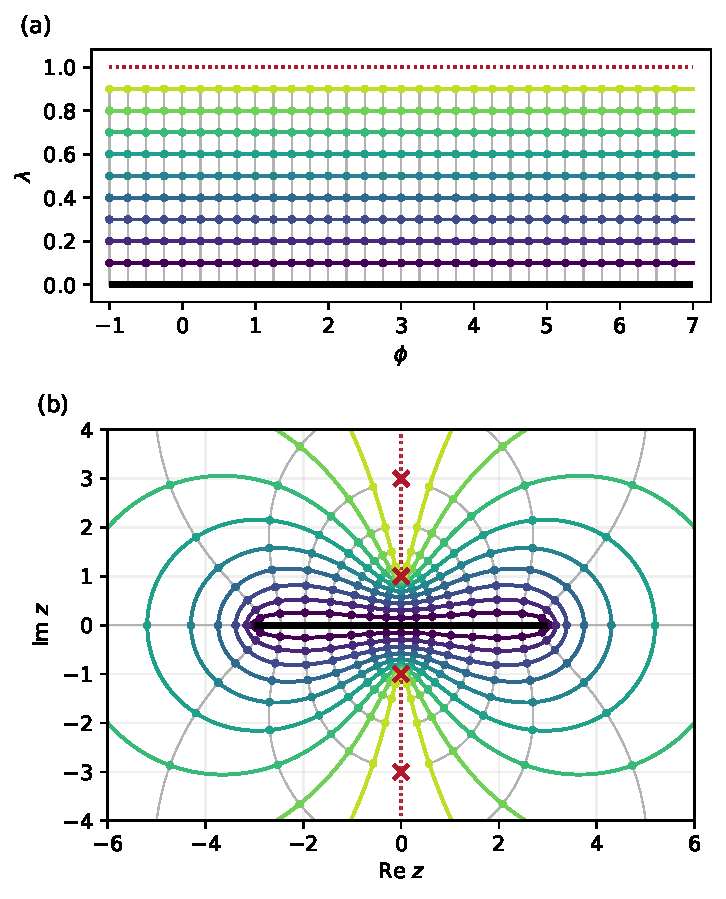
\includegraphics[width=\columnwidth]{bubble_tn_dumbbells.pdf}
  \caption{The dumbbell family. (a) The strip $\zeta=\phi+i\tau\lambda$: the levels $\lambda=0.1,\ldots,0.9$ (colored lines) between the band ($\lambda=0$, black) and the level $\lambda=1$ (dotted) and the grid $\phi_j=-1+8j/N$ for $N=32$ (dots). (b) Its image under $\omega$: the dumbbells $C_\lambda$ (same colors) around the band $[-3,3]$ and the nodes $z_j=\omega_\lambda(\phi_j)$. The poles of the Fermi function at $\pm i,\pm3i$ ($\beta=\pi$) lie on the level $\lambda=1$, the imaginary axis beyond $\pm i$ (dotted).}
  \label{fig:dumbbells}
\end{figure}

\subsection{Properties of the dumbbell map}
\label{sec:dumbbell_map}

We write $\omega_\lambda(\phi)=\omega(\phi+i\tau\lambda)$: $\phi$ is the position along a contour and $\lambda$ its \emph{level}, where $\tau=K'(k)/K(k)$, with $k=(L-1)/(L+1)$ and $L=\sqrt{1+(E\beta/\pi)^2}$. The function $\sd$ satisfies $\sd(u+2K)=-\sd(u)$, $\sd(u+2iK')=-\sd(u)$ and $\sd(-u)=-\sd(u)$, and its Taylor coefficients are real, so
\begin{equation}
  \begin{gathered}
  \omega(\zeta+8)=\omega(\zeta),\qquad \omega(\zeta+4)=-\omega(\zeta),\\
  \omega(2-\zeta)=\omega(\zeta),\qquad \overline{\omega(\zeta)}=\omega(\bar\zeta)=\omega(2-\bar\zeta).
  \end{gathered}
  \label{eq:symmetries}
\end{equation}
In terms of $\phi$ and $\lambda$: period 8 in $\phi$; $\omega_\lambda(\phi+4)=-\omega_\lambda(\phi)$; and $\omega_\lambda(2-\phi)=\overline{\omega_\lambda(\phi)}$, so the lower half of every contour is the mirror image of its upper half.

For fixed $\lambda\in(0,1)$, $\phi\mapsto\omega_\lambda(\phi)$, $\phi\in[-1,7)$, traces a closed curve $C_\lambda$ once, the \emph{dumbbell at level $\lambda$}. Its shape follows from the values at $\lambda\to0$ and $\lambda=1$:
\begin{itemize}
  \item $\lambda\to0^+$: $\omega$ is real and runs $0\to E\to0\to-E\to0$ for $\phi=-1\to1\to3\to5\to7$. The contour collapses onto the segment $[-E,E]$: $\phi\in(-1,1)\cup(5,7)$ is the upper half ($\Imag\omega>0$), $\phi\in(1,5)$ the lower half. The \emph{tips} are $\phi=1$ and $\phi=5$ ($\omega=\pm E$), and the curve crosses the imaginary axis at $\phi=-1\equiv7$ and $\phi=3$ ($\omega=0$). In increasing $\phi$ the curve is traversed clockwise.
  \item $\lambda=1$: $\omega(\phi+i\tau)$ is purely imaginary with $\lvert\Imag\omega\rvert\ge\pi/\beta$ ($\omega(-1+i\tau)=i\pi/\beta$, and $\omega\to\infty$ at $\phi=1,5$, where $\sd$ has its poles). The level-1 ``contour'' is the imaginary axis beyond the first poles, $\{\Real z=0,\ \lvert\Imag z\rvert\ge\pi/\beta\}$.
\end{itemize}
Every level $0<\lambda<1$ lies between the segment and the level-1 curve. The strip $0<\lambda<2$ is mapped by $\omega$ onto $\mathbb C\setminus[-E,E]$ (the level $2-\lambda$ gives the mirror image $-\overline{C_\lambda}$ of $C_\lambda$, the same curve), and $\lambda=2$ is the segment again.

The map is tied to the temperature through the poles of the Fermi function $f(z)=1/(e^{\beta z}+1)$, at the fermionic Matsubara frequencies $i\omega_n=i(2n+1)\pi/\beta$ (Sec.~\ref{sec:bubble}). With $\kappa/\kappa'=E\beta/\pi$ the two closest to the real axis, $\pm i\pi/\beta$, sit at the ends of the level-1 curve, and then all poles lie on it. This is the choice of modulus of Lin, Lu, Ying and E, $L=\sqrt{1+(E\beta/\pi)^2}$. Every contour $C_\lambda$ with $0<\lambda<1$ separates the segment from all poles of $f$.

The Jacobian of the map follows from $v=\frac K2(\zeta+1)$ and $\frac{d}{dv}\sd v=\cn v/\dn^2v$:
\begin{equation}
  \begin{gathered}
  J(\zeta)\equiv\frac{\partial\omega}{\partial\phi}=E\kappa'\,\frac K2\,\frac{\cn v}{\dn^2v},\qquad
  \frac{\partial\omega}{\partial\lambda}=i\tau\,J,\\
  J^2=\Big(\frac{K\kappa'\beta}{2\pi}\Big)^2\Big(\frac{\pi^2}{\beta^2}+\omega^2\Big)(E^2-\omega^2),
  \end{gathered}
  \label{eq:jacobian}
\end{equation}
the second relation because $\omega$ is analytic in $\zeta=\phi+i\tau\lambda$, the third from $\dn^2v=1/(1+\beta^2\omega^2/\pi^2)$ and $\cn^2v=(1-\omega^2/E^2)/(1+\beta^2\omega^2/\pi^2)$. We write $J_\lambda(\phi)=J(\phi+i\tau\lambda)$. For $0<\lambda<1$, $J_\lambda$ has no zeros on $C_\lambda$; on the segment it is $J_0(\varepsilon)=\frac{K\kappa'\beta}{2\pi}\sqrt{(E^2-\varepsilon^2)(\pi^2/\beta^2+\varepsilon^2)}$, which vanishes like $\sqrt{E-\lvert\varepsilon\rvert}$ at the edges, so the nodes cluster at the edges of the segment like Chebyshev points [Fig.~\ref{fig:dumbbells}(b)].

Every $z$ off the segment and the level-1 curve lies on exactly one dumbbell $C_{\lambda'}$, and we call $\lambda(z)\equiv\lambda'$ the \emph{level} of $z$.

$C_\lambda$ crosses the imaginary axis at $\omega_\lambda(-1)=iE\kappa'\,\sd(K'\lambda\,|\,\kappa'^2)$ and $\omega_\lambda(3)=-\omega_\lambda(-1)$, by $\sd(iy\,|\,\kappa^2)=i\,\sd(y\,|\,\kappa'^2)$; these are the lowest point of its upper half and the highest point of its lower half. The highest and lowest points of $C_\lambda$ follow from \eqref{eq:jacobian} (Fig.~\ref{fig:height}). Along $C_\lambda$ the tangent $J$ is horizontal where $J^2$ is real and positive. Since $J^2\propto(\pi^2/\beta^2+\omega^2)(E^2-\omega^2)$, the imaginary part of $J^2$ for $\omega=x+iy$ is proportional to $2xy[E^2-\pi^2/\beta^2-2(x^2-y^2)]$, which off the axes vanishes on the hyperbola $x^2-y^2=c^2$, $c^2=(E^2-\pi^2/\beta^2)/2$, where $J^2$ is positive. The highest and lowest points of a dumbbell of height $H$ are therefore
\[
  z=\pm\sqrt{c^2+H^2}\pm iH ,
\]
and since the dumbbells are nested, $C_\lambda$ stays within $\lvert\Imag z\rvert<H$ exactly when $\lambda<\lambda^*(H)\equiv\lambda\big(\sqrt{c^2+H^2}+iH\big)$. We call $H_\lambda$ the height of $C_\lambda$, so that its top is $\sqrt{c^2+H_\lambda^2}+iH_\lambda$ and $\lambda^*(H_\lambda)=\lambda$.

\begin{figure}[t]
  \centering
  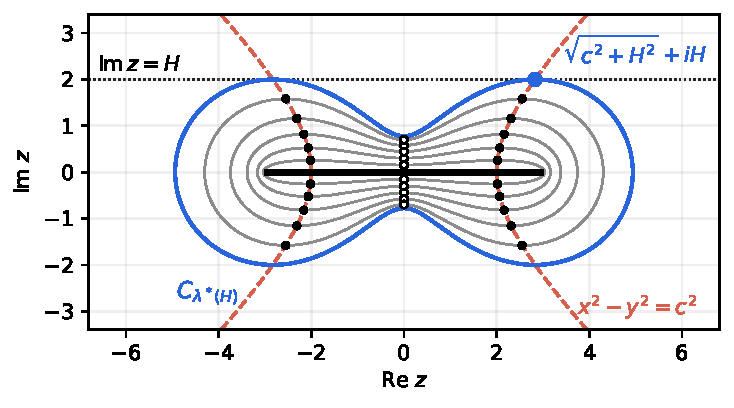
\includegraphics[width=\columnwidth]{dumbbell_height.pdf}
  \caption{Highest and lowest points of the dumbbells, for $E=3$ and $\beta=\pi$. The extreme points (dots) of every $C_\lambda$ (grey) lie on the hyperbola $x^2-y^2=c^2$ (dashed), where the tangent $J$ is horizontal, and the open circles mark where they cross the imaginary axis. The dumbbell $C_{\lambda^*(H)}$ (blue) touches the line $\Imag z=H$ (dotted) at its highest points $\pm\sqrt{c^2+H^2}+iH$, here for $H=\nu_1$, and it crosses the imaginary axis at $\pm\omega_\lambda(-1)=\pm iE\kappa'\,\sd(K'\lambda\,|\,\kappa'^2)$ (blue open circles); every $C_\lambda$ with $\lambda<\lambda^*(H)$ stays below the line.}
  \label{fig:height}
\end{figure}

The contour formula \eqref{eq:contour_w} on the nodes $z_j$ needs $G$ at the shifted points $z_j\pm w_k$, which lie on the translated copies $C_\lambda\pm w_k$ of the contour. Each shifted point has a level; the lowest one,
\begin{equation}
  \lambda'_{\min}(\lambda,\mu)=\min_{j,k}\ \lambda\big(z_j\pm w_k\big),
  \label{eq:lammin}
\end{equation}
measures how close the copies come to the segment ($\lambda'_{\min}>0$) and whether they stay outside $C_\lambda$ ($\lambda'_{\min}>\lambda$). By the symmetry $w_{k+N/2}=-w_k$ the sets $\{z_j+w_k\}$ and $\{z_j-w_k\}$ coincide. The copies come closest to the segment when $w_k$ is where $C_\mu$ crosses the imaginary axis and $z_j$ at the highest or lowest point of $C_\lambda$. Raising $\mu$ or lowering $\lambda$ raises $\lambda'_{\min}$, and $\lambda'_{\min}>\lambda$ holds for $\mu$ above a threshold $\mu_{\rm fwd}(\lambda)$, roughly for $\lambda\lesssim\mu/2$.

\section{The formula behind the network}
\label{sec:formula}

\subsection{The bubble}
\label{sec:bubble}

Momenta are on the grid $q=2\pi m/N_q$, $m=0,\ldots,N_q-1$, and all momentum sums and shifts are modulo $2\pi$. The temperature is $1/\beta$; the fermionic and bosonic Matsubara frequencies are
\begin{equation}
  \omega_n=\frac{(2n+1)\pi}{\beta},\qquad \nu_m=\frac{2\pi m}{\beta},\qquad n,m\in\mathbb Z,
  \label{eq:matsubara}
\end{equation}
and the Fermi function is
\begin{subequations}
\label{eq:fermi}
\begin{align}
  f(z)&=\frac1{e^{\beta z}+1},\label{eq:fermi_def}\\
  f(z+i\nu_m)&=f(z),\label{eq:fermi_periodic}\\
  \Res_{z=i\omega_n}f&=-\frac1\beta .\label{eq:fermi_res}
\end{align}
\end{subequations}
\begin{figure}[t]
  \centering
  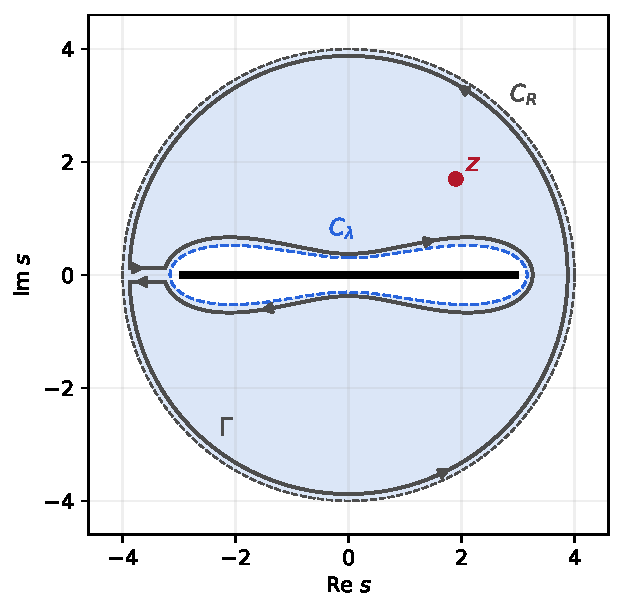
\includegraphics[width=0.85\columnwidth]{cauchy_region.pdf}
  \caption{Cauchy's integral formula, the first equality in \eqref{eq:lehmann}, for $G$ at a point $z$ outside the dumbbell $C_\lambda$ (dashed, $\lambda=0.2$). $G$ is analytic in the shaded region between $C_\lambda$ and the circle $C_R$ (dashed), and its singularities lie on the band $[-3,3]$ (black). A horizontal cut on the left, from $C_\lambda$ to $C_R$, makes the region simply connected. Its counterclockwise boundary $\Gamma$ (dark), drawn slightly inside it, is a single closed contour that encloses $z$ and no singularity of $G$, so Cauchy's formula on it gives $G(z)$. The two sides of the cut are traversed in opposite directions and cancel, and $\Gamma$ reduces to $C_R$ counterclockwise and $C_\lambda$ clockwise; the clockwise orientation turns $1/(s-z)$ into the $1/(z-s)$ of \eqref{eq:lehmann}. As $R\to\infty$ the $C_R$ integral vanishes.}
  \label{fig:cauchy}
\end{figure}

The one-particle Green function $G_q(z)$ is analytic off the band $[-E,E]$, and $G_q(z)\sim1/z$ for $z\to\infty$. For any function $\psi$ analytic inside and on $C_\lambda$, shrinking $C_\lambda$ onto the band, where it runs along $\varepsilon-i0^+$ from left to right and back along $\varepsilon+i0^+$, gives
\begin{equation}
  \frac1{2\pi i}\oint_{C_\lambda}ds\,G_q(s)\,\psi(s)=\int_{-E}^{E}d\varepsilon\,A_q(\varepsilon)\,\psi(\varepsilon),
  \label{eq:shrink}
\end{equation}
with the spectral function
\begin{equation}
  \begin{aligned}
  A_q(\varepsilon)&=\frac{G_q(\varepsilon-i0^+)-G_q(\varepsilon+i0^+)}{2\pi i}\\
  &=-\frac1\pi\Imag G_q(\varepsilon+i0^+),
  \end{aligned}
  \label{eq:specfn}
\end{equation}
the jump of $G_q$ across the band. For $z$ outside $C_\lambda$, $\psi(s)=1/(z-s)$ gives the spectral representation
\begin{equation}
  G_q(z)=\frac1{2\pi i}\oint_{C_\lambda}ds\,\frac{G_q(s)}{z-s}=\int_{-E}^{E}d\varepsilon\,\frac{A_q(\varepsilon)}{z-\varepsilon},
  \label{eq:lehmann}
\end{equation}
where the first equality is Cauchy's formula on the contour $\Gamma$ of Fig.~\ref{fig:cauchy}, which consists of a circle $C_R$, counterclockwise, and of $C_\lambda$, clockwise; the $C_R$ integral vanishes as $R\to\infty$. With $\psi(s)=e^{-ist}$, \eqref{eq:shrink} gives the time representation, the real-time Green function
\begin{equation}
  \bar g_q(t)=\frac1{2\pi i}\oint_{C_\lambda}ds\,G_q(s)\,e^{-ist}=\int_{-E}^{E}d\varepsilon\,A_q(\varepsilon)\,e^{-i\varepsilon t}.
  \label{eq:gbar}
\end{equation}
Conversely, since $\varepsilon$ is real, $1/(z-\varepsilon)$ is a time integral: with $\sigma=\operatorname{sgn}\Imag z$,
\begin{equation}
  \frac1{z-\varepsilon}=-i\sigma\int_{-\infty}^{\infty}dt\,\theta(\sigma t)\,e^{i(z-\varepsilon)t},
  \label{eq:laplace_z}
\end{equation}
and inserting it into \eqref{eq:lehmann} gives $G_q$ in terms of $\bar g_q$,
\begin{equation}
  G_q(z)=-i\sigma\int_{-\infty}^{\infty}dt\,\theta(\sigma t)\,e^{izt}\,\bar g_q(t).
  \label{eq:ginv}
\end{equation}
The integral converges for every $z$ off the real axis, since $\lvert\bar g_q(t)\rvert\le\int d\varepsilon\,\lvert A_q(\varepsilon)\rvert$, and $G_q$ is the Fourier transform of $-i\sigma\theta(\sigma t)\,\bar g_q(t)$, the retarded Green function for $\sigma=1$ and the advanced one for $\sigma=-1$. With $\psi(s)=f(s)\,e^{ist}$, \eqref{eq:shrink} gives the occupied real-time Green function $g_q(t)$, obtained from $\bar g_q(-t)$ by replacing $G_q$ with $fG_q$ and $A_q$ with $fA_q$.

As an example we take a tight-binding chain with nearest-neighbour hopping,
\begin{equation}
  \begin{gathered}
  \varepsilon_q=3\cos q,\qquad G_q(z)=\frac1{z-\varepsilon_q},\\
  A_q(\varepsilon)=\delta(\varepsilon-\varepsilon_q),
  \end{gathered}
  \label{eq:model}
\end{equation}
at the inverse temperature $\beta=\pi$; its band is $[-3,3]$, and the bubble has its cut on $[-6,6]$. For this model the bubble is the Lindhard function \eqref{eq:lindhard}, the reference for every accuracy quoted.

The bubble reads
\begin{equation}
  \begin{aligned}
  \chi_Q(i\nu_m)&=\frac1{N_q\beta}\sum_{q,n}G_q(i\omega_n)\,G_{q+Q}(i\omega_n+i\nu_m)\\
  &=\frac1{N_q}\sum_q\frac1\beta\sum_nh(i\omega_n),
  \end{aligned}
  \label{eq:bubble_def}
\end{equation}
with
\begin{equation}
  h(z)=G_q(z)\,G_{q+Q}(z+i\nu_m).
  \label{eq:h}
\end{equation}
The Matsubara sum converges absolutely because the summand is $O(\omega_n^{-2})$. By \eqref{eq:lehmann} the poles of $h$, which merge into cuts for a continuous spectrum, lie on the band $[-E,E]$ of the real axis, from $G_q(z)$, and on the band moved down by $\nu_m$, from $G_{q+Q}(z+i\nu_m)$. These lie at the heights $0$ and $-\nu_m$, even multiples of $\pi/\beta$, while the poles $i\omega_n$ of $f$ lie at odd multiples. So $h$ is regular at the poles of $f$, and with the residue $-1/\beta$ of $f$ in \eqref{eq:fermi_res}, $\Res_{z=i\omega_n}[f(z)h(z)]=-h(i\omega_n)/\beta$. Hence
\begin{equation}
  \frac1\beta\sum_nh(i\omega_n)=-\sum_n\Res_{z=i\omega_n}\big[f(z)\,h(z)\big].
  \label{eq:matsum_residues}
\end{equation}
\subsection{The contour formula}
\label{sec:contour}

\begin{figure}[t]
  \centering
  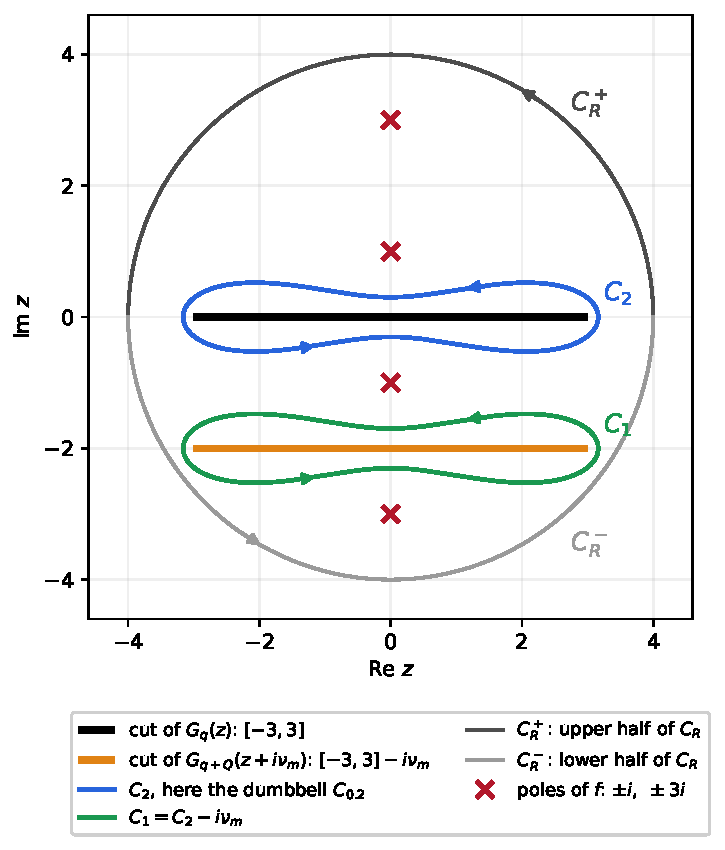
\includegraphics[width=\columnwidth]{contours_C.pdf}
  \caption{The decomposition of the circle $C_R$ that leads to \eqref{eq:residues_cuts}, for $\beta=\pi$ and $m=1$ ($\nu_1=2$). The poles of $h$ of \eqref{eq:h} lie on the band $[-3,3]$ of the real axis (black), from $G_q(z)$, and on the band moved down by $\nu_m$ (orange), from $G_{q+Q}(z+i\nu_m)$. Horizontal lines at the distance $\eta$ above and below them cut the disk into five regions, whose counterclockwise boundaries $C_+$, $C_3$, $C_2$, $C_1$ and $C_-$ are drawn slightly inside them. $C_3$ encloses the band, $C_1$ the shifted band, and $C_+$, $C_2$, $C_-$ the poles of $f$. Each line is traversed in both directions, so the five contours add up to $C_R$. The dashed curves are the dumbbells $C_\lambda$ and $C_\lambda-i\nu_m$, here for $\lambda=0.2$, into which $C_3$ and $C_1$ are deformed.}
  \label{fig:contours}
\end{figure}

Let $C_R$ be the counterclockwise circle centred at the origin with radius $R$, halfway between two poles of $f$. For $R\to\infty$ it contains both the poles of $h$, at $\Imag z=0$ and $\Imag z=-\nu_m$, and those of $f$, and elsewhere inside it $fh$ is analytic. For $m>0$, as shown in Fig.~\ref{fig:contours}, the contour integral over $C_R$ can be rewritten as a sum of contour integrals over $C_R=C_-+C_1+C_2+C_3+C_+$. These are the counterclockwise boundaries of the five regions into which horizontal lines, at the distance $\eta<\pi/\beta$ above and below the poles of $h$, cut the disk; each line is traversed twice, in opposite directions, and drops out. $C_3$ encloses the poles of $h$ on the real axis and $C_1$ those on the shifted line, while $C_-$, $C_2$ and $C_+$ enclose only poles of $f$. As $R\to\infty$, the integrals of $fh/(2\pi i)$ over $C_-$, $C_2$ and $C_+$ give minus the right-hand side of \eqref{eq:matsum_residues}, while the integral over $C_R$ vanishes, because $h=O(z^{-2})$ and $f$ stays bounded on $C_R$, so that
\begin{equation}
  \begin{aligned}
  \sum_n\Res_{z=i\omega_n}\big[f(z)\,h(z)\big]={}&-\frac1{2\pi i}\oint_{C_1}f\,h\,dz\\
  &-\frac1{2\pi i}\oint_{C_3}f\,h\,dz .
  \end{aligned}
  \label{eq:residues_cuts}
\end{equation}
The contour integrals over $C_3$ and $C_1$ can be deformed into integrals over the dumbbells $C_\lambda$ and $C_\lambda-i\nu_m$ (dashed lines in Fig.~\ref{fig:contours}) as long as $C_\lambda$ leaves out the shifted band $[-E,E]-i\nu_m$. The dumbbell $C_\lambda$ stays within $\lvert\Imag z\rvert<\nu_m$ for $\lambda<\lambda^*(\nu_m)$ (Sec.~\ref{sec:dumbbell_map}), so the deformations are safe for $\lambda<\lambda^*(\nu_m)$, and since $\nu_m\ge\nu_1$, the bound for $m=1$ covers every $m>0$. By the change of variables $z\to z-i\nu_m$ in the integral over $C_\lambda-i\nu_m$ and by \eqref{eq:fermi_periodic}, we have, at $w=i\nu_m$,
\begin{equation}
  \begin{aligned}
  \chi_Q(w)={}&\frac1{N_q}\sum_q\frac1{2\pi i}\oint_{C_\lambda}dz\;f(z)\,G_q(z)\\
  &\times\Big[G_{q+Q}(z+w)+G_{q-Q}(z-w)\Big].
  \end{aligned}
  \label{eq:contour_w}
\end{equation}
At $w=i\nu_m$ and for $\lambda<\lambda^*(\nu_m)$, the factors $f(z)\,G_{q\pm Q}(z\pm w)$ are analytic inside and on $C_\lambda$. Inserting \eqref{eq:lehmann}, Cauchy's formula turns \eqref{eq:contour_w} into
\begin{equation}
  \begin{aligned}
  \chi_Q(w)={}&\frac1{N_q}\sum_q\int_{-E}^{E}\!d\varepsilon\int_{-E}^{E}\!d\varepsilon'\,A_q(\varepsilon)\,A_{q+Q}(\varepsilon')\\
  &\times\frac{f(\varepsilon)-f(\varepsilon')}{w+\varepsilon-\varepsilon'} ,
  \end{aligned}
  \label{eq:spectral}
\end{equation}
with $w=i\nu_m$. Equation \eqref{eq:spectral} does not depend on $\lambda$, is analytic in $w$ off the interval $[-2E,2E]$ of the differences $\varepsilon'-\varepsilon$ and vanishes as $\lvert w\rvert\to\infty$, so it is the analytic continuation $\chi_Q(w)$ of the bubble.

\begin{figure}[t]
  \centering
  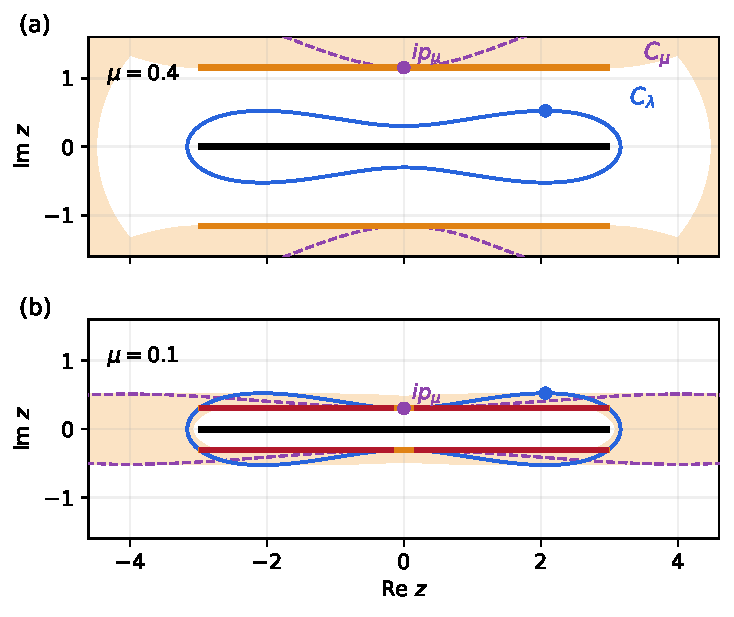
\includegraphics[width=\columnwidth]{cloud_condition.pdf}
  \caption{The condition $\lambda<\Lambda(\mu,\beta)$ for $\lambda=0.2$, $\mu=0.4$ and $\beta=\pi$, with the vertical scale stretched $1.5$ times. The thin lines are the shifted cuts $[-3,3]\pm w$ for points $w$ on $C_\mu$ (dots); for all $w$ on $C_\mu$ they sweep the cloud $[-3,3]\pm C_\mu$ (shaded), the zone that $C_\lambda$ must avoid. Near the band its edge comes from the points $\pm ip_\mu$ where $C_\mu$ crosses the imaginary axis, and the dot on $C_\lambda$ is its highest point. The point $ip_\mu$ lies above the highest point of $C_\lambda$, so $C_\lambda$ lies in the hole of the cloud and \eqref{eq:contour_w} gives $\chi_Q(w_k)$.}
  \label{fig:cloud}
\end{figure}

Now let $w$ be a general complex number. The same steps give \eqref{eq:spectral} as long as $C_\lambda$ leaves out the shifted cuts $[-E,E]\mp w$, where $G_{q\pm Q}(z\pm w)$ is singular. For $w=w_k\in C_\mu$, where $C_\mu=C_\mu(2E,\beta/2)=2\,C_\mu(E,\beta)$ is a dumbbell which encloses $[-2E,2E]$ and leaves out the poles $i\nu_m$, $m\ne0$, of the Bose function, the shifted cuts sweep the set $[-E,E]\pm C_\mu$, the ``cloud'' in Fig.~\ref{fig:cloud}, so \eqref{eq:contour_w} holds on $C_\mu$ when the cloud lies outside $C_\lambda$. This happens when the top of $C_\lambda$ lies below the point $ip_\mu$ where $C_\mu$ crosses the imaginary axis, with $p_\mu=2\,\Imag\omega(-1+i\tau\mu)$ (Sec.~\ref{sec:dumbbell_map}):
\[
  H_\lambda<p_\mu=2E\kappa'\,\sd(K'\mu\,|\,\kappa'^2) .
\]
In terms of levels this reads $\lambda<\Lambda(\mu,\beta)$, where $\Lambda(\mu,\beta)=\lambda^*(p_\mu)=\lambda\big(\sqrt{c^2+p_\mu^2}+ip_\mu\big)$. Since $p_\mu<\nu_1\le\nu_m$ and the level $\lambda^*(H)$ grows with $H$, $\Lambda(\mu,\beta)=\lambda^*(p_\mu)<\lambda^*(\nu_m)$, and the only condition on $\lambda$ becomes $\lambda<\Lambda(\mu,\beta)$.

\subsection{The bubble as a product in time}
\label{sec:time}

The data are the values of $G$ on $C_\lambda$, while \eqref{eq:contour_w} needs $G_{q\pm Q}$ at the shifted points $z\pm w$, off the contour. The spectral form \eqref{eq:spectral} is a bilinear form in the spectral functions with the kernel
\begin{equation}
  \Psi_w(\varepsilon,\varepsilon')=\frac{f(\varepsilon)-f(\varepsilon')}{w+\varepsilon-\varepsilon'},
  \label{eq:kernel_psi}
\end{equation}
and \eqref{eq:shrink}, applied in each variable, gives
\begin{equation}
  \begin{aligned}
  &\frac1{(2\pi i)^2}\oint_{C_\lambda}dz\oint_{C_\lambda}ds\,G_q(z)\,G_{q'}(s)\,\Psi(z,s)\\
  &\quad=\int_{-E}^{E}d\varepsilon\int_{-E}^{E}d\varepsilon'\,A_q(\varepsilon)\,A_{q'}(\varepsilon')\,\Psi(\varepsilon,\varepsilon')
  \end{aligned}
  \label{eq:shrink2}
\end{equation}
for every $\Psi$ analytic in both variables inside and on $C_\lambda$. The right side depends on $\Psi$ only through its values on the band, and with $\Psi=\Psi_w$ and $q'=q+Q$, summed over $q$ and divided by $N_q$, it is the bubble \eqref{eq:spectral}. The Cauchy route of Appendix~\ref{app:cauchy} applies \eqref{eq:shrink2} to $\Psi_w$ itself, which requires $\Psi_w$ to be analytic inside $C_\lambda$, that is, the copies $C_\lambda\pm w$ outside $C_\lambda$, $\lambda'_{\min}>\lambda$ in \eqref{eq:lammin}; on the nodes $\Psi_w$ is then a dense tensor in $z_j$, $z_m$ and $w_k$, compressed in Appendix~\ref{sec:tucker}. Appendix~\ref{app:kernel_time} obtains the compressed tensor from the time route, where this condition is not needed. The time route first writes $\Psi_w$ on the band as an integral over time of products of exponentials, one factor per variable, and applies \eqref{eq:shrink2} to each product, which is analytic inside $C_\lambda$ for every time.

\begin{figure*}[t]
  \centering
  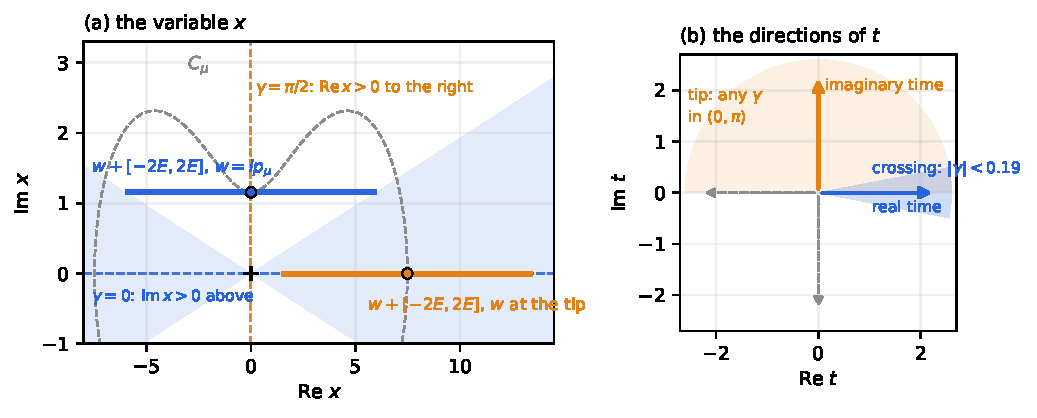
\includegraphics[width=0.82\textwidth]{laplace_geometry.pdf}
  \caption{The geometry of the time representation \eqref{eq:laplace}, for $E=3$, $\beta=\pi$ and $\mu=0.4$. (a) The variable $x$. For the direction $\gamma$ the formula holds in the half-plane $\Imag(xe^{i\gamma})>0$, bounded by the line through the origin at the angle $-\gamma$: the real axis for real time (blue dashed) and the imaginary axis for imaginary time (orange dashed). In the bubble $x=w+\varepsilon-\varepsilon'$ fills the segment $w+[-2E,2E]$, drawn at the crossing $w=ip_\mu$ of $C_\mu$ (blue) and at its right tip (orange), with $C_\mu$ dashed. The lines through the origin that miss the first segment fill the blue double wedge, of half-angle $\arctan(p_\mu/2E)=0.19$, so real time works there. The second segment lies on the real axis, and the lines that miss it are all the others, best the imaginary axis. (b) The corresponding directions of $t$: within 0.19 of real time at the crossing (blue), anywhere in $(0,\pi)$ at the tip, with imaginary time in the middle (orange). All admissible directions give the same $1/x$.}
  \label{fig:laplace_geometry}
\end{figure*}

For complex $x$ and a direction $\gamma$ in the complex $t$ plane,
\begin{equation}
  \frac1x=-i\int_{\mathcal L_\gamma}dt\,e^{ixt},\qquad\Imag(xe^{i\gamma})>0,
  \label{eq:laplace}
\end{equation}
where $\mathcal L_\gamma=\{e^{i\gamma}\tau:\tau\ge0\}$ is the half-line from $0$ to $\lim_{r\to\infty}re^{i\gamma}$; on it $t=e^{i\gamma}\tau$ and $dt=e^{i\gamma}d\tau$. The direction $\gamma=0$ is real time and $\gamma=\pi/2$ imaginary time, and for $\gamma=0$ and $\gamma=\pi$, \eqref{eq:laplace} is \eqref{eq:laplace_z}. With $t=e^{i\gamma}\tau$, \eqref{eq:laplace} is the elementary integral of $e^{i(xe^{i\gamma})\tau}$ over $\tau>0$: the direction rotates $x$ by $e^{i\gamma}$ into the upper half-plane, so for a fixed $\gamma$ the formula holds in the half-plane of $x$ bounded by the line through the origin at the angle $-\gamma$ (Fig.~\ref{fig:laplace_geometry}). Since $e^{ixt}$ is entire in $t$, Cauchy's theorem on the sector between two admissible directions shows that they give the same $1/x$. The inverse relation is a residue: for real $t$, $(2\pi)^{-1}\int dx\,e^{-ixt}/x$ along a line above the origin is $-i\theta(t)$, since for $t>0$ the contour closes below and encloses the pole at $x=0$, and for $t<0$ it closes above and encloses nothing. With $x=w+\varepsilon-\varepsilon'$ the integrand $e^{iwt}\,e^{i\varepsilon t}\,e^{-i\varepsilon't}$ has one factor per variable, so in time the kernel is diagonal, a delta in $t$, which is the copy tensor of Fig.~\ref{fig:time_network}. Inserted into \eqref{eq:spectral}, \eqref{eq:laplace} makes the integrals over $\varepsilon$ and $\varepsilon'$ factorize into $\bar g_q$ of \eqref{eq:gbar} and $g_q$ at complex $t$, where their contour forms still hold. The term with $f(\varepsilon)$ gives $g_q(t)\,\bar g_{q+Q}(t)$, and the term with $f(\varepsilon')$ gives $\bar g_q(-t)\,g_{q+Q}(-t)$, so the bubble becomes a product in time,
\begin{equation}
  \begin{aligned}
  \chi_Q(w)={}&-\frac{i}{N_q}\sum_q\int_{\mathcal L_\gamma}dt\,e^{iwt}\\
  &\times\big[g_q(t)\,\bar g_{q+Q}(t)-\bar g_q(-t)\,g_{q+Q}(-t)\big],
  \end{aligned}
  \label{eq:time_bubble}
\end{equation}
exact when $\Imag(we^{i\gamma})>2E\lvert\sin\gamma\rvert$, that is, when the segment $w+[-2E,2E]$ of the values of $x$ lies in the half-plane of $\gamma$. Summed over $q$, the second product is the first one in the direction $\gamma+\pi$, read at $-Q$; for $\gamma=0$ it is the complex conjugate of the first one at $-Q$, since $\bar g_q(-t)=\bar g_q(t)^*$ and $g_q(-t)=g_q(t)^*$ for real $t$, $A_q$ and $f$ being real on the band. The functions $\bar g_q$ and $g_q$ are integrals of the data over $C_\lambda$, so $G$ is never needed off the contour.

\begin{figure}[!htbp]
  \centering
  \includegraphics[width=\columnwidth]{margins.pdf}
  \caption{The conditions of the time route for $\lambda=0.2$ and $\mu=0.4$ ($E=3$, $\beta=\pi$), at the crossing $w=ip_\mu$ with real time (a) and at the right tip of $C_\mu$ with imaginary time (b), with $C_\mu$ dashed. Shifted by $w$: the segment $w+[-2E,2E]$ (black), the set $w+[-E,E]+D_\lambda$ (orange), with $D_\lambda$ the region inside $C_\lambda$, and the set $w+D_\lambda+D_\lambda$ (grey). The dashed line bounds the half-plane of the direction, and its tinted side is excluded. Exact, stable and bounded mean that the black, the orange and the grey set lie in the half-plane; the margin of \eqref{eq:margin} is the distance of the orange set, 0.63 and 1.32, and the grey set lies at 0.11 and 1.16 (dotted). The vertical scale is stretched.}
  \label{fig:margins}
\end{figure}

The conditions can be read off the integrand of \eqref{eq:time_bubble}, with $t=e^{i\gamma}\tau$. The kernel $e^{iwt}$ decays like $e^{-\Imag(we^{i\gamma})\tau}$. On $C_\lambda$ the exponentials of the node sums obey $\lvert e^{\pm ist}\rvert\le e^{H_\lambda(\gamma)\tau}$, where $H_\lambda(\gamma)=\max_{s\in C_\lambda}\Imag(se^{i\gamma})$ is the height of $C_\lambda$ in the direction $ie^{-i\gamma}$, while $\bar g_q$ and $g_q$ grow only like $e^{E\lvert\sin\gamma\rvert\tau}$, as on the band. The node sums therefore carry rounding errors of relative size $e^{(H_\lambda(\gamma)-E\lvert\sin\gamma\rvert)\tau}$ times the machine precision, and the kernel damps these errors when
\begin{equation}
  \Imag(we^{i\gamma})>H_\lambda(\gamma)+E\lvert\sin\gamma\rvert,
  \label{eq:margin}
\end{equation}
that is, when $w$ lies beyond every point $\varepsilon+s$, with $\varepsilon\in[-E,E]$ and $s\in C_\lambda$, in the direction $ie^{-i\gamma}$. We call the difference of the two sides the margin. Read in this way, the direction $\gamma$ is the real-time route applied to the rotated frequencies $ze^{i\gamma}$ and $we^{i\gamma}$, and $H_\lambda(\gamma)$ is the height of the rotated contour $e^{i\gamma}C_\lambda$. Figure~\ref{fig:margins} shows the conditions as three nested sets, shifted by $w$: the segment $w+[-2E,2E]$ decides whether \eqref{eq:time_bubble} is exact, the set $w+[-E,E]+D_\lambda$, with $D_\lambda$ the region inside $C_\lambda$, whether its node sums are stable, with the margin as its distance from the line, and the set $w+D_\lambda+D_\lambda$ whether the gauge of Sec.~\ref{sec:quadrature} keeps every intermediate number bounded. Real time, $\gamma=0$ and $\gamma=\pi$, serves the upper and lower halves of $C_\mu$, where \eqref{eq:margin} reads $\Imag w>H_\lambda$ and $\Imag w<-H_\lambda$. Imaginary time, $\gamma=\pi/2$ and $\gamma=3\pi/2$, serves the regions around the right and left tips, where it reads $\Real w>E+\omega_\lambda(1)$ and $\Real w<-E-\omega_\lambda(1)$, with $\omega_\lambda(1)=E\operatorname{nc}(K'\lambda\,|\,\kappa'^2)$, $\operatorname{nc}=1/\cn$, the tip of $C_\lambda$ on the positive real axis. At the point $ip_\mu$ the margin of real time is $p_\mu-H_\lambda$, positive under the condition $\lambda<\Lambda(\mu,\beta)$ of \eqref{eq:contour_w}. The Cauchy route needs the stronger condition $\lambda'_{\min}>\lambda$.

The spectral form is not needed to obtain \eqref{eq:time_bubble}. Inserting \eqref{eq:laplace} with $x=w+z-s$ directly into the double contour integral \eqref{eq:shrink2} with $\Psi=\Psi_w$ gives the same product, with the same contour forms of $\bar g_q$ and $g_q$, but only where every pair of points $z$, $s$ of $C_\lambda$ gives a decaying exponential, that is, where $w+D_\lambda+D_\lambda$ lies in the half-plane of $\gamma$; this also makes $\Psi_w$ analytic inside $C_\lambda$, as \eqref{eq:shrink2} requires. At the crossing $ip_\mu$ it is the condition $p_\mu>2H_\lambda$ of the Cauchy route. The detour through the spectral form proves \eqref{eq:time_bubble} under the weaker conditions on the segment and on $w+[-E,E]+D_\lambda$, and the second test of Sec.~\ref{sec:tests} lies between the two. There the products of the terms of the node sums grow faster than $e^{iwt}$ decays, the sums cancel down to their values on the band, and the gauge of Sec.~\ref{sec:quadrature} shares the growth between the leaves and the Laplace train.

No single direction serves all of $C_\mu$, and neither does any discretization of \eqref{eq:time_bubble} whose times and weights do not depend on $w$. Such a discretization is an entire function $g(w)$, while $\chi_Q$ has its cut inside $C_\mu$. With $C_\mu$ traversed counterclockwise, $\oint_{C_\mu}dw\,w\,g(w)=0$, while $\oint_{C_\mu}dw\,w\,\chi_Q(w)=2\pi i\,c_2$, where
\begin{equation}
  \begin{aligned}
  c_2={}&\frac1{N_q}\sum_q\int_{-E}^{E}d\varepsilon\int_{-E}^{E}d\varepsilon'\,A_q(\varepsilon)\,A_{q+Q}(\varepsilon')\\
  &\times\big[f(\varepsilon)-f(\varepsilon')\big](\varepsilon'-\varepsilon)
  \end{aligned}
  \label{eq:c2}
\end{equation}
is the coefficient of $w^{-2}$ in the expansion of \eqref{eq:spectral} at large $w$. Since $f$ decreases and $A_q\ge0$, $c_2>0$ unless $\chi_Q$ vanishes, and
\begin{equation}
  \max_{w\in C_\mu}\lvert\chi_Q(w)-g(w)\rvert\ge\frac{2\pi c_2}{L_\mu R_\mu},
  \label{eq:entire_bound}
\end{equation}
with $L_\mu$ the length of $C_\mu$ and $R_\mu=\max_{C_\mu}\lvert w\rvert$. The weights must therefore depend on the output point, and the direction of the time integral is the cheapest such dependence.

\begin{figure}[!htbp]
  \centering
  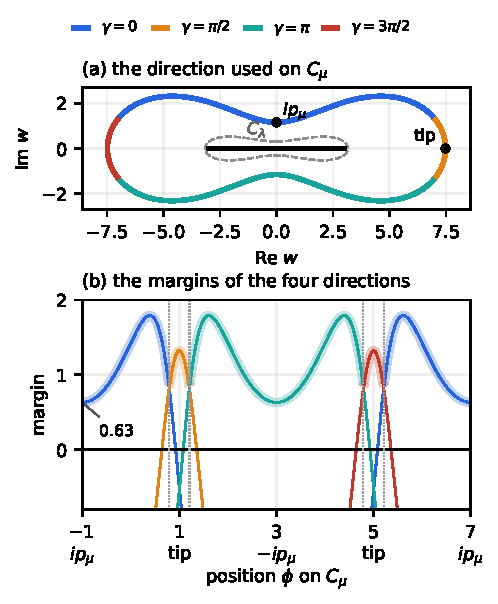
\includegraphics[width=\columnwidth]{directions.pdf}
  \caption{The partition of \eqref{eq:one_formula} on $C_\mu$ for $\lambda=0.2$ and $\mu=0.4$ ($E=3$, $\beta=\pi$, $N=512$). (a) $C_\mu$ coloured by the direction with the largest margin, with $C_\lambda$ dashed: real time $\gamma=0$ on the 229 points of the upper half and $\gamma=\pi$ on the 229 of the lower half, imaginary time $\gamma=\pi/2$ and $3\pi/2$ on the 27 points around each tip. (b) The margins $m_\gamma(w)=\Imag(we^{i\gamma})-H_\lambda(\gamma)-E\lvert\sin\gamma\rvert$ of \eqref{eq:margin} along $C_\mu$, with $\phi$ the position on $C_\mu$; the shaded band marks the largest one. Since $H_\lambda(0)=H_\lambda(\pi)=H_\lambda$ and $H_\lambda(\pm\pi/2)=\omega_\lambda(1)$, they are $\pm\Imag w-H_\lambda$ and $\pm\Real w-E-\omega_\lambda(1)$. The mask is $P_\gamma(w)=1$ where $m_\gamma$ is the largest, so the arcs meet where $C_\mu$ crosses the lines $\lvert\Imag w\rvert-H_\lambda=\lvert\Real w\rvert-E-\omega_\lambda(1)$ (dotted), where both margins are 0.82. The smallest margin on $C_\mu$, 0.63, is at the crossings $\pm ip_\mu$.}
  \label{fig:directions}
\end{figure}

Let $X_Q$ be the part of the bubble with $f(\varepsilon)$,
\begin{equation}
  X_Q(w)=\frac1{N_q}\sum_q\int_{-E}^{E}d\varepsilon\int_{-E}^{E}d\varepsilon'\,\frac{f(\varepsilon)\,A_q(\varepsilon)\,A_{q+Q}(\varepsilon')}{w+\varepsilon-\varepsilon'}.
  \label{eq:xq}
\end{equation}
In the term of \eqref{eq:spectral} with $f(\varepsilon')$, the substitution $q\to q-Q$ together with $\varepsilon\leftrightarrow\varepsilon'$ gives $X_{-Q}(-w)$, so $\chi_Q(w)=X_Q(w)+X_{-Q}(-w)$. For every direction with $\Imag(we^{i\gamma})>2E\lvert\sin\gamma\rvert$, \eqref{eq:laplace} turns \eqref{eq:xq} into $X_Q(w)=-i\int_{\mathcal L_\gamma}dt\,e^{iwt}\,Y_Q(t)$, with $Y_Q(t)=N_q^{-1}\sum_qg_q(t)\,\bar g_{q+Q}(t)$; \eqref{eq:time_bubble} is this formula applied to both terms with the same direction. Let $P_\gamma(w)$, $\gamma\in\{0,\pi/2,\pi,3\pi/2\}$, be a partition of unity on $C_\mu$, $\sum_\gamma P_\gamma(w)=1$, with $P_\gamma(w)=0$ wherever the margin of $\gamma$ is below a fixed $m_0>0$; it exists when every point of $C_\mu$ has a direction with a margin of at least $m_0$. The simplest choice is a mask, $P_\gamma(w)=1$ for the direction with the largest margin at $w$ and $0$ for the others (Fig.~\ref{fig:directions}). Then
\begin{equation}
  \begin{aligned}
  \chi_Q(w)&=X_Q(w)+X_{-Q}(-w),\\
  X_Q(w)&=-i\sum_\gamma P_\gamma(w)\int_{\mathcal L_\gamma}dt\,e^{iwt}\,Y_Q(t),
  \end{aligned}
  \label{eq:one_formula}
\end{equation}
at every point of $C_\mu$, with one fixed set of directions. Each direction is used only where \eqref{eq:laplace} converges, so \eqref{eq:one_formula} is exact, and only where its margin is at least $m_0$, so the rounding error of each term is of the order of the machine precision divided by $m_0$. By \eqref{eq:xq}, $X_Q$ is analytic off $[-2E,2E]$, like $\chi_Q$, and every direction gives the same function where it is used, so the partition changes only how $X_Q$ is computed.

\subsection{The time domain on the nodes}
\label{sec:quadrature}

The time functions $g_q$ and $\bar g_q$ are integrals over $C_\lambda$. Parametrize $C_\lambda$ by $\phi$: $z=\omega_\lambda(\phi)$, $dz=J_\lambda(\phi)\,d\phi$. The parametrization is clockwise, so for any $F$ analytic near the contour
\begin{equation}
  \frac1{2\pi i}\oint_{C_\lambda}F(z)\,dz=-\frac1{2\pi i}\int_{-1}^{7}d\phi\;J_\lambda(\phi)\,F\big(\omega_\lambda(\phi)\big).
\end{equation}
The integrand is 8-periodic in $\phi$, and the trapezoidal rule on the uniform grid $\phi_j=-1+j\,\Delta\phi$, $j=0,\ldots,N-1$, with $\Delta\phi=8/N$, is $\Delta\phi\sum_j$. The nodes are $z_j=\omega_\lambda(\phi_j)$, and the bubble is computed at the points $w_k=2\,\omega(\phi_k+i\tau\mu)$ of $C_\mu$ on the same grid. With the Fermi function in the integrand it gives
\begin{equation}
  \begin{gathered}
  \frac1{2\pi i}\oint_{C_\lambda}f\,F\,dz\approx\sum_{j=0}^{N-1}c_j\,F(z_j),\\
  c_j=d_j\,f(z_j),\qquad d_j=-\frac{\Delta\phi}{2\pi i}J_\lambda(\phi_j).
  \end{gathered}
  \label{eq:weights}
\end{equation}
For every $F$ that is analytic outside $C_\lambda$ and $O(z^{-2})$ at infinity, the residue theorem between $C_\lambda$ and a large circle, as in Sec.~\ref{sec:contour}, gives $\sum_jc_jF(z_j)\approx\beta^{-1}\sum_nF(i\omega_n)$: the $N$ nodes with the weights $c_j$ replace the Matsubara frequencies. Without the Fermi function the rule reads $\frac1{2\pi i}\oint_{C_\lambda}F\,dz\approx\sum_md_m\,F(z_m)$. The $c_j$ depend on $j$, $\lambda$ and $\beta$ only, never on $w$, $q$ or $G$, and the Fermi function is evaluated only at the nodes of $C_\lambda$. Both sets of weights are smooth in $\phi_j$ (rank 6 to 8 as quantics tensor trains, Appendix~\ref{sec:qtt}). The quadrature error falls exponentially with $N$, like $e^{-\alpha Nd}$ \eqref{eq:rate}, where $d$ is the distance in level from $C_\lambda$ to the nearest singularity of the integrand (Appendix~\ref{app:trap}).

The two rules applied to $g_q$ and $\bar g_q$ give the time functions from the data, at real or complex $t$,
\begin{equation}
  \begin{aligned}
  g_q(t)&\approx\sum_jc_j\,G_q(z_j)\,e^{iz_jt},\\
  \bar g_q(t)&\approx\sum_md_m\,G_q(z_m)\,e^{-iz_mt},\\
  \lvert e^{\pm iz_jt}\rvert&\le e^{H_\lambda(\gamma)\lvert t\rvert}.
  \end{aligned}
  \label{eq:gt_nodes}
\end{equation}
For each of the four directions $\gamma_a$ the integral over $\tau=\lvert t\rvert$ in \eqref{eq:one_formula} is replaced by a rule $\int_0^{T_a}d\tau\,h(\tau)\approx\sum_p\varpi_p\,h(\tau_p)$. At the points where $P_{\gamma_a}(w_k)>0$ the integrand decays at least like $e^{-d_a\tau}$, with $d_a$ the smallest value of $\Imag(w_ke^{i\gamma_a})-2E\lvert\sin\gamma_a\rvert$ there, and $T_a$ is the time at which $e^{-d_aT_a}$ reaches the target accuracy. In real time the integrand oscillates with frequencies up to $\max_k\lvert\Real w_k\rvert+2E$, which Gauss-Legendre panels of equal length resolve. In imaginary time it is a sum of exponentials with rates between $d_a$ and $d_a+4E$, and the panels double in length from the origin. The time leg $p$ runs over the four rules, with the times $t_p=e^{i\gamma_p}\tau_p$.

A function given on the $N$ nodes of $C_\lambda$ has the discrete Fourier representation
\begin{equation}
  \begin{aligned}
  G_q(z_j)&=\sum_{n}\hat g_{q,n}\,e^{i\pi n\phi_j/4},\\
  \hat g_{q,n}&=\frac1N\sum_{j=0}^{N-1}G_q(z_j)\,e^{-i\pi n\phi_j/4},
  \end{aligned}
  \label{eq:ghat}
\end{equation}
where $n$ runs over any $N$ consecutive integers (we use the two's-complement range $-N/2\le n<N/2$); both relations are exact on the grid. Since $e^{i\pi n\phi_j/4}=e^{-i\pi n/4}e^{2\pi inj/N}$, the coefficient $\hat g_{q,n}$ is $e^{i\pi n/4}/N$ times the standard FFT of the data.

\begin{figure*}[tp]
  \centering
  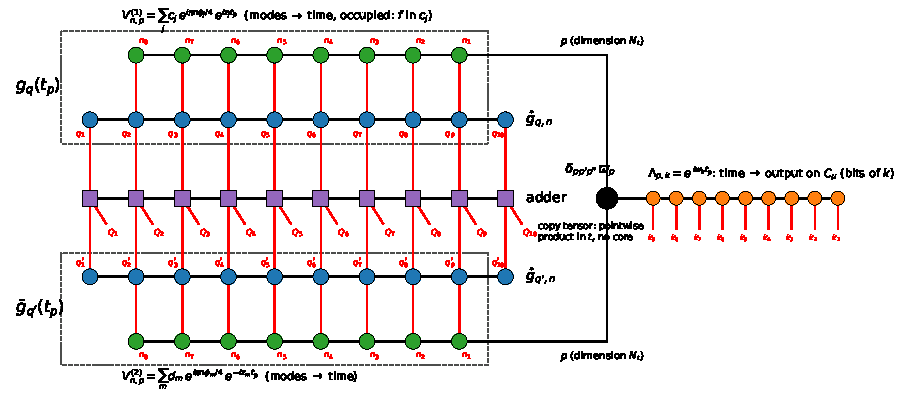
\includegraphics[width=\textwidth]{time_network.pdf}
  \caption{The time-domain network, in the conventions of Fig.~\ref{fig:contraction} (red legs are contracted, bits most significant first). Upper branch: the input train $\hat g_{q,n}$ (blue), its $n$ legs contracted with the train $V^{(1)}_{n,p}$ (green), which carries the modes to the time points $t_p$ and contains the Fermi function through $c_j$; the result is $A_{q,p}$, the function $g_q(t_p)$ in the gauge of \eqref{eq:vandermonde}, a train over the bits of $q$ with the time leg $p$. Lower branch: the same with $V^{(2)}$ (weights $d_m$, no $f$, opposite sign in the exponent), which gives $B_{q',p}$, the function $\bar g_{q'}(t_p)$. The adder (purple) sums $q$ and $q'$ with the transfer momentum $Q$ open. The two time legs meet at a copy tensor carrying the weights $\varpi_p$, the product in time, and the Laplace train $\Lambda_{p,k}$ (orange) sends the time leg to the output points of $C_\mu$ (bits of $k$). The time leg runs over the rules of the four directions; the labels give the leading factors of the tensors \eqref{eq:vandermonde}, without the gauge and the partition. The network gives $X_Q(w_k)$, and $\chi_Q(w_k)$ of \eqref{eq:time_nodes} is $X_Q(w_k)$ plus the same train read at $-Q$ and $k+N/2$.}
  \label{fig:time_network}
\end{figure*}

In these modes the time functions are linear in the data. With a gauge $h_p$, for instance $h_p=H_\lambda(\gamma_p)$, the network is built from the tensors
\begin{equation}
  \begin{aligned}
  V^{(1)}_{n,p}&=\sum_jc_j\,e^{i\pi n\phi_j/4}\,e^{iz_jt_p-h_p\tau_p},\\
  V^{(2)}_{n,p}&=\sum_md_m\,e^{i\pi n\phi_m/4}\,e^{-iz_mt_p-h_p\tau_p},\\
  \Lambda_{p,k}&=-i\,e^{i\gamma_p}\,P_{\gamma_p}(w_k)\,e^{iw_kt_p+2h_p\tau_p},
  \end{aligned}
  \label{eq:vandermonde}
\end{equation}
in which \eqref{eq:one_formula} reads
\begin{equation}
  \begin{aligned}
  A_{q,p}&=\sum_n\hat g_{q,n}V^{(1)}_{n,p},\qquad B_{q,p}=\sum_n\hat g_{q,n}V^{(2)}_{n,p},\\
  Y_p(Q)&=\frac1{N_q}\sum_qA_{q,p}\,B_{q+Q,p},\\
  X_Q(w_k)&=\sum_p\varpi_p\,\Lambda_{p,k}\,Y_p(Q),\\
  \chi_Q(w_k)&=X_Q(w_k)+X_{-Q}(w_{k+N/2}),
  \end{aligned}
  \label{eq:time_nodes}
\end{equation}
since $-w_k=w_{k+N/2}$ by \eqref{eq:symmetries}. The gauge cancels between the leaves and $\Lambda$. With $h_p=H_\lambda(\gamma_p)$ every term of the node sums is at most $\max_j\lvert c_jG_q(z_j)\rvert$, the entries of $V^{(1)}$ and $V^{(2)}$ are at most $\sum_j\lvert c_j\rvert$ and $\sum_m\lvert d_m\rvert$, and $\lvert\Lambda_{p,k}\rvert\le1$ wherever $\Imag(w_ke^{i\gamma_p})\ge2H_\lambda(\gamma_p)$; where this fails on part of an arc, a smaller $h_p$ shares the remaining growth between the leaves and $\Lambda$. Since the leaves are bounded, the input $\hat g$ needs no weights $1/s_n$, unlike in the Cauchy route, and the modes with $s_n$ below the target accuracy can be dropped (Appendix~\ref{sec:decay}). The matrices $V^{(1)}$, $V^{(2)}$ and $\Lambda$ depend only on the geometry, the time rules and the partition. Each mask $P_\gamma(w_k)$ is the indicator of the arc of $C_\mu$ where $\gamma$ has the largest margin, an interval of $k$. Its ends follow from the switch point $\phi^*$ between the crossing and the right tip, where $\Real w(\phi)-E-\omega_\lambda(1)=\Imag w(\phi)-H_\lambda$ with $w(\phi)=2\omega(\phi+i\tau\mu)$, and from the symmetries $w(2-\phi)=w(\phi)^*$ and $w(\phi+4)=-w(\phi)$, which put the other switch points at $2-\phi^*$, $4+\phi^*$ and $6-\phi^*$. The indicator of an interval is an exact train of bond at most 3 (Appendix~\ref{sec:qtt}), so the mask enters $\Lambda$ without approximation. In the network of Fig.~\ref{fig:time_network} the input train $\hat g$ is contracted with $V^{(1)}$ and $V^{(2)}$, the adder forms $Y_p(Q)$, a copy tensor multiplies by $\varpi_p$, and the Laplace train $\Lambda_{p,k}$ sends the time leg to the output points $w_k$. The result is the train $X_Q(w_k)$. The second term of \eqref{eq:time_nodes} is the same train read at $-Q$ and $k+N/2$, that is, after the reflection $Q\to-Q$ of Appendix~\ref{sec:qtt} and a NOT on the most significant bit of $k$, and the two trains are added as in Appendix~\ref{app:sum}.

\section{Tests}
\label{sec:tests}

\begin{table*}[t]
\caption{The time network and the Cauchy route for the model \eqref{eq:model} with $\lambda=0.2$, $N=512$ and $N_q=1024$, compared with the Lindhard function at all points of $C_\mu$ and all transfer momenta. The error is $\max_{Q,k}\lvert\chi-\chi_{\rm exact}\rvert/\max_{Q,k}\lvert\chi_{\rm exact}\rvert$, and the largest entries of the trains are relative to $\max\lvert\chi_{\rm exact}\rvert$. The bonds are the largest bonds of TT-SVDs of the dense trains at $10^{-10}$ with the criterion \eqref{eq:trunc}; $A$, $B$ and $Y$ carry the time leg $p$ (time network) or a Tucker leg (Cauchy route) at their first site. Real time alone uses $\gamma=0$ on the upper half of $C_\mu$ and $\gamma=\pi$ on the lower half.}
\label{tab:time}
\centering\small
\setlength{\tabcolsep}{6pt}
\begin{tabular}{@{}lccccc@{}}
\toprule
 & \multicolumn{2}{c}{time network} & \multicolumn{2}{c}{Cauchy route} & real time alone \\
 & $\mu=0.4$ & $\mu=0.25$ & $\mu=0.4$ & $\mu=0.25$ & $\mu=0.4$ \\
\midrule
time points or Tucker ranks & 1024 & 2048 & $(31,33,44)$ & $(67,70,103)$ & 512 \\
smallest margin on $C_\mu$ & 0.63 & 0.11 & & & $-0.52$ \\
error & $4.6\times10^{-14}$ & $1.3\times10^{-13}$ & $1.7\times10^{-7}$ & $5.3\times10^{-2}$ & 0.11 \\
largest entry of $A$, $Y$ & 4.6, 2.3 & 3.5, 1.7 & 47, 0.93 & & \\
rank of $\Lambda$ over $(p,k)$ & 176 & 257 & & & 24 \\
largest bond of $A$, $B$, $Y$ & 70, 68, 55 & 102, 100, 68 & 46, 47, 40 & & \\
largest bond of $\chi$ & 40 & 62 & 38 & & \\
\bottomrule
\end{tabular}
\end{table*}

We test the network on the model \eqref{eq:model} with $\lambda=0.2$, $N=512$ and $N_q=1024$, at $\mu=0.4$ and at $\mu=0.25$. The second value lies below $\mu_{\rm fwd}(0.2)=0.36$, so the copies $C_\lambda\pm w_k$ overlap $C_\lambda$ and the Cauchy route of Appendix~\ref{app:cauchy} fails, while $\lambda<\Lambda(\mu,\beta)$ still holds. The reference is the Lindhard function \eqref{eq:lindhard} at all 512 points of $C_\mu$ and all transfer momenta. The tensors are built densely in double precision. Each direction has 8 Gauss-Legendre panels of 32 points at $\mu=0.4$ and 16 panels at $\mu=0.25$, with $d_aT_a=30$, and the partition takes the direction with the largest margin. The gauge is $h_p=H_\lambda(\gamma_p)$ at $\mu=0.4$; at $\mu=0.25$, where $p_\mu<2H_\lambda$, it is lowered to $h_p=0.40$ in real time and $3.15$ in imaginary time. Table~\ref{tab:time} collects the results. Its bonds are those of TT-SVDs of the dense tensors, while Table~\ref{tab:steps} gives those of the recompressed trains of the Cauchy route.

The time network gives the bubble to $4.6\times10^{-14}$ of its maximum at $\mu=0.4$ and $1.3\times10^{-13}$ at $\mu=0.25$, at every point of $C_\mu$, the tips included; where $\lvert\chi_Q\rvert$ exceeds $10^{-3}$ of its maximum, the relative error is below $10^{-11}$. The trains $A$, $B$, $Y$ and $X$ stay below five times the largest $\lvert\chi_Q\rvert$, and the entries of the leaves stay below 2 at $\mu=0.4$ and below 44 at $\mu=0.25$, while without the gauge the node sums reach $10^{39}$ and $10^{142}$. The Cauchy route gives $1.7\times10^{-7}$ at $\mu=0.4$, the accuracy of its kernel compressed at $10^{-8}$, and fails at $\mu=0.25$. Real time alone, $\gamma=0$ on the upper half and $\gamma=\pi$ on the lower half, is accurate on most of $C_\mu$ but errs by $0.11$ of the maximum at the tips, where the integrand does not decay, and more time points do not reduce this error. The bound \eqref{eq:entire_bound} quantifies why imaginary time is needed there. At $\mu=0.4$ and $Q=\pi$, $c_2=3.75$, $L_\mu=35.6$ and $R_\mu=7.49$, so any formula entire in $w$ errs by at least $0.088$, that is $41\,\%$ of $\max_k\lvert\chi_Q\rvert$; at the other transfer momenta tested and at $\mu=0.25$ the bound lies between 14 and $43\,\%$.

The bonds of the result $\chi$ are those of the Cauchy route, 40 against 38 at $\mu=0.4$, since the two routes represent the same tensor. At $N_q=64$ the two results differ by $1.7\times10^{-7}$, the error of the Cauchy kernel, and their bonds are identical at $10^{-8}$ and $10^{-6}$; the part $X_Q$ alone has the widest bond 40 at $10^{-10}$, against 27 for $\chi_Q$. The directions enter only the Laplace train, which is built once from the geometry, like the Tucker core, and never from $G$, and its projection of Appendix~\ref{app:kernel_time} is a dense map without blocks, of rank 55 at $10^{-10}$. The intermediate trains carry the time leg and are larger: the Laplace train has rank 176 over $(p,k)$ at $\mu=0.4$, against the 44 output modes of the Cauchy route, and the largest bonds of $A$ and $Y$ are 70 and 55 against 46 and 40. The core, however, is diagonal: the time leg sits at the first site of $A$, $B$ and $Y$, where the Cauchy route carries its Tucker legs, and the adder step carries a leg of 1024 points instead of the leg $(a,c)$ of $B'$, of dimension $r_1r_3=1364$. No HOSVD and no Cauchy sums over the nodes are needed. With the input on the window $s_n\ge10^{-10}$, 131 modes, the error is $4.7\times10^{-14}$, and on $s_n\ge10^{-6}$, 78 modes, it is $4.6\times10^{-9}$ ($1.5\times10^{-8}$ at $\mu=0.25$), so the input window follows the target accuracy. A smooth partition, with weights proportional to the square of the margin above $m_0=0.3$ or $0.5$, gives the same accuracy with the longer windows $T_a\le57$ or $43$ and a Laplace train of rank 205 or 187.

\section{Toward a GW scheme on contours}
\label{sec:gw}

The bubble is the first step of a GW scheme in which every frequency-dependent quantity, $G$, $\chi$, the screened interaction $W$ and the self-energy $\Sigma$, is stored on a contour, and every step is a tensor-network operation with a controlled error. This section gives the equations of such a loop, the conditions on its contours, the self-energy in the form of Sec.~\ref{sec:time}, the loop in train form, its memory and cost against a dense scheme, the continuation of its result to the real axis, and the order in which the pieces can be built and tested. The numbers come from the dense tests of Secs.~\ref{sec:gw_tests} to~\ref{sec:gw_continuation}.

\subsection{The loop}
\label{sec:gw_loop}

\begin{figure}[t]
  \centering
  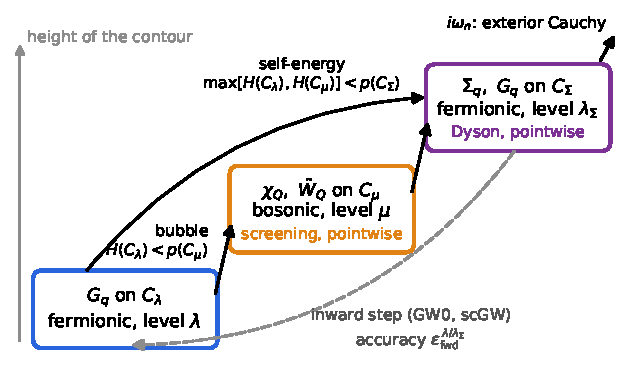
\includegraphics[width=\columnwidth]{gw_loop.pdf}
  \caption{The GW loop on contours. The boxes are placed at the heights of their contours, which rise along $G\to\chi\to\Sigma$. Each forward step, the bubble and the self-energy, needs the condition written next to it, while screening and Dyson's equation are pointwise. In G0W0 the chain ends on $C_\Sigma$, and the values at the Matsubara frequencies follow from the exterior Cauchy formula \eqref{eq:ext_cauchy}. GW0 and scGW close the loop with the inward step \eqref{eq:inward} (dashed), whose accuracy is the forward accuracy raised to the level ratio.}
  \label{fig:gw_loop}
\end{figure}

For electrons with two spin directions and an interaction $v_Q$, the polarization is $\Pi_Q=2\chi_Q$, with $\chi_Q$ the bubble \eqref{eq:bubble_def} of the current $G$, and the screened interaction and its screened part are
\begin{equation}
  \begin{aligned}
  W_Q&=\frac{v_Q}{1-v_Q\Pi_Q},\\
  \tilde W_Q&=W_Q-v_Q=\frac{v_Q^2\,\Pi_Q}{1-v_Q\Pi_Q}.
  \end{aligned}
  \label{eq:screening}
\end{equation}
The self-energy is $\Sigma_q(z)=\Sigma^{\rm H}+\Sigma^{\rm x}_q+\Sigma^{\rm c}_q(z)$. The Hartree term $\Sigma^{\rm H}=v_0\rho$ shifts the chemical potential, and the exchange and correlation terms are
\begin{equation}
  \begin{aligned}
  \Sigma^{\rm x}_q&=-\frac1{N_q}\sum_Qv_Q\,\rho_{q-Q},\\
  \Sigma^{\rm c}_q(i\omega_n)&=-\frac1{N_q\beta}\sum_{Q,m}G_{q-Q}(i\omega_n-i\nu_m)\,\tilde W_Q(i\nu_m),
  \end{aligned}
  \label{eq:sigma_def}
\end{equation}
where $\rho_q=\sum_jc_jG_q(z_j)=\int d\varepsilon\,f(\varepsilon)A_q(\varepsilon)$ is the occupation, a node sum with the weights \eqref{eq:weights} that needs no convergence factor, and $\rho=(2/N_q)\sum_q\rho_q$ is the density. Dyson's equation $G_q(z)=1/[z-\varepsilon_q-\Sigma_q(z)]$, with $\varepsilon_q$ measured from the chemical potential, closes the loop, and the chemical potential is fixed by $\rho$. In G0W0 the chain $G_0\to\chi\to W\to\Sigma\to G$ runs once. In GW0 $W$ is kept and $\Sigma$ and $G$ are iterated, and in self-consistent GW (scGW) the bubble is recomputed from the dressed $G$ as well (Fig.~\ref{fig:gw_loop}).

In train form every object is one train over the bits of its momentum and the bits of its contour, either the point index $k$ or the Fourier mode $n$ of \eqref{eq:ghat}, which the DFT MPO of Appendix~\ref{app:qft} converts at bond 11. The bubble and the self-energy are the network of Fig.~\ref{fig:time_network}. A dense time leg of $N_t$ points at the first site of $A$ and $B$ would make the adder zip-up cost about $N_t(\chi_A\chi_BdD_W)^2$, so the leg is compressed over $p$ to the rank of the leaves, and the network becomes that of Appendix~\ref{app:cauchy} with the kernel \eqref{eq:kernel_time}; the diagonal core serves the dense tests. Screening and Dyson's equation are the Newton products of Sec.~\ref{sec:gw_reciprocal}. The inward step is the DFT, the diagonal multiplier $e^{\alpha(\lambda_\Sigma-\lambda)n}$, the window $n\le n_{\max}$ and the DFT back. In two's complement $n=-n_12^{R-1}+\sum_{i\ge2}n_i2^{R-i}$, so the multiplier is a product of one factor per bit and its MPO has bond 1; the window has bond 2, and a smooth window $e^{-(n/n_{\max})^8}$ bond 8. The density is the contraction with the train of the weights $c_j$, of bond 6 to 8. No step inverts a matrix, and the result of every step is one train on all of its contour. A GW0 iteration needs about ten zip-ups, the reciprocals, six MPO applications and three sums, each followed by a recompression; scGW adds the bubble and the screening.

\subsection{Supports and contours}
\label{sec:gw_contours}

Each object is stored on a contour around its support. The support of $G$ is a segment $[-E_G,E_G]$, the band at the start, which grows with the support of $\Sigma$. That of $\chi$ is $[-2E_G,2E_G]$, and that of $\tilde W_Q$ is $[-\Omega_W,\Omega_W]$, which also covers the poles of $W$ outside the particle-hole continuum, at the zeros of $1-v_Q\Pi_Q$ on the real axis. On a finite lattice such a zero exists above every continuum. For an even band and $v_Q>0$ its position $\omega$ satisfies $\omega^2\le4E_G^2+2v_Qc_2$, with $c_2$ of \eqref{eq:c2}, and the coefficient of $w^{-2}$ in $\tilde W_Q$, $2v_Q^2c_2$, detects weight left outside the segment. The support of $\Sigma^{\rm c}$ is $[-E_G-\Omega_W,E_G+\Omega_W]$. In the iterated schemes $G$ and $\Sigma$ share one fermionic family on $[-E_G,E_G]$, with $E_G\ge E+\Omega_W$, so that Dyson's equation is pointwise, and $\chi$ and $\tilde W$ share one bosonic family, which encloses the pole of the Bose function at the origin and no other. On a finite lattice the pairs with $\varepsilon_{q+Q}=\varepsilon_q$ contribute $f'(\varepsilon_q)$ to $\Pi_Q(i\nu_0)$ and nothing at $\nu_m\neq0$. The node sum $\chi_Q(0)=N_q^{-1}\sum_q\sum_jc_jG_q(z_j)G_{q+Q}(z_j)$ gives this Matsubara value, while a spectral representation of $\tilde W$ misses it.

Each forward step has one condition, the one of \eqref{eq:contour_w}: the contours of its inputs lie below the point where the contour of its output crosses the imaginary axis. With $H(C)$ the height of a contour $C$ and $p(C)$ the height of its crossing, the bubble needs $H(C_\lambda)<p(C_\mu)$, and the self-energy of Sec.~\ref{sec:gw_sigma}, computed on a contour $C_\Sigma$ of the fermionic family at a level $\lambda_\Sigma$, needs $\max[H(C_\lambda),H(C_\mu)]<p(C_\Sigma)$. Screening, Dyson's equation, exchange and density are pointwise operations or node sums and need no condition. Since $H(C)\ge p(C)$, the levels rise along $G\to\chi\to\Sigma$. In G0W0 this costs nothing: $\Sigma$ and $G$ are known on $C_\Sigma$, and their values at the Matsubara frequencies, or anywhere outside $C_\Sigma$, follow from the exterior Cauchy formula \eqref{eq:ext_cauchy}. In GW0 and scGW, $\Sigma$ must be brought down from $C_\Sigma$ to the contour $C_\lambda$ of $G$. Within a family this is the level multiplier \eqref{eq:multiplier}, which multiplies the mode $n$ by $e^{\alpha(\lambda_\Sigma-\lambda)n}$. If the forward steps give $\Sigma$ on $C_\Sigma$ to the accuracy $\varepsilon_{\rm fwd}$, the modes beyond $\ln(1/\varepsilon_{\rm fwd})/(\alpha\lambda_\Sigma)$ are below the forward error, and the step reaches
\begin{equation}
  \varepsilon_{\rm in}\approx\varepsilon_{\rm fwd}^{\,\lambda/\lambda_\Sigma}.
  \label{eq:inward}
\end{equation}
The level ratio $\lambda_\Sigma/\lambda$ is therefore the price of the loop.

\begin{figure}[t]
  \centering
  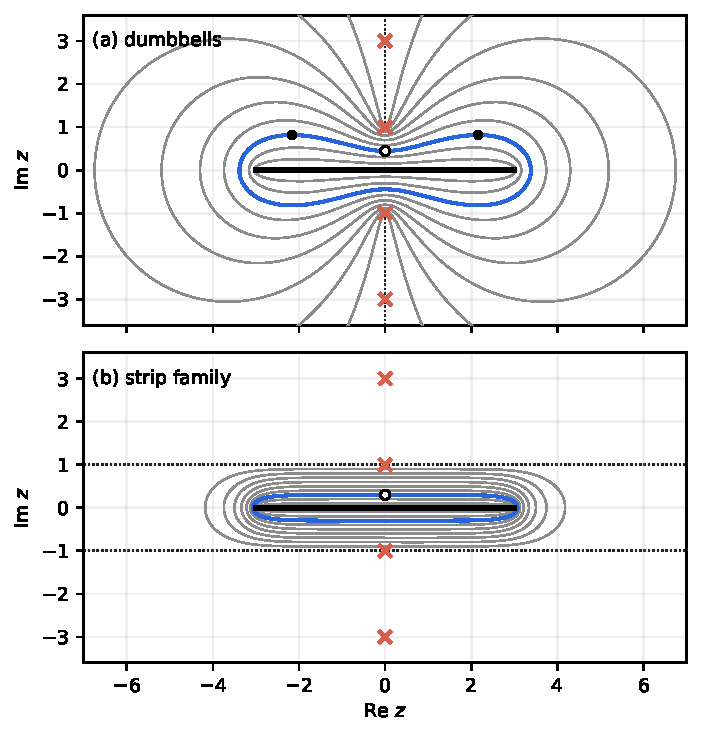
\includegraphics[width=\columnwidth]{gw_families.pdf}
  \caption{The dumbbells (a) and the strip family (b) for $E=3$ and $\beta=\pi$, at the levels $\lambda=0.1,\ldots,0.9$ (grey) with $\lambda=0.3$ in blue, the band $[-3,3]$ (black), the poles $\pm i$, $\pm3i$ of $f$ (crosses) and the level-1 curves (dotted): the imaginary axis beyond $\pm i$ for the dumbbells, the lines $\Imag z=\pm1$ for the strip family. The dots mark the highest points and the open circles the crossings of the imaginary axis. On the dumbbell at $\lambda=0.3$ the top lies at 1.8 times the crossing; on the strip family the two coincide, $H=p=0.30$.}
  \label{fig:gw_families}
\end{figure}

On the dumbbells the top of a contour lies above its crossing, $H(C_\lambda)>p(C_\lambda)$, and the ratio $H/p$ grows with $E$, so the chain needs a large level ratio. A second family has $H=p$ (Fig.~\ref{fig:gw_families}). With $k=\tanh(\beta E/2)$, $k'^2=1-k^2$, and $K$ and $K'$ the complete elliptic integrals of parameters $k^2$ and $k'^2$, the map
\begin{equation}
  z(\zeta)=\frac2\beta\operatorname{artanh}\Big[k\,\sn\Big(\frac K2(\zeta+1)\,\Big|\,k^2\Big)\Big]
  \label{eq:strip_map}
\end{equation}
sends the strip $\zeta=\phi+i\tau\lambda$ of Sec.~\ref{sec:dumbbell}, with $\tau=2K'/K$, onto the plane strip $\lvert\Imag z\rvert<\pi/\beta$ cut along $[-E,E]$. The line $\lambda=0$ goes to the segment, and the line $\lambda=1$ to the lines $\Imag z=\pm\pi/\beta$, which pass through the first poles $\pm i\pi/\beta$ of $f$; for a bosonic family the same map with $\beta/2$ gives lines through the first poles $\pm2\pi i/\beta$ of the Bose function. The level curves of this map, the strip family, have their highest point on the imaginary axis, at
\begin{equation}
  H_\lambda=p_\lambda=\frac2\beta\arctan\big[k\,\operatorname{sc}(K'\lambda\,|\,k'^2)\big],
  \label{eq:strip_height}
\end{equation}
with $\operatorname{sc}=\sn/\cn$, and their tips at $\pm(2/\beta)\operatorname{artanh}[k\operatorname{nd}(K'\lambda\,|\,k'^2)]$, with $\operatorname{nd}=1/\dn$. The decay rate $\alpha=\pi\tau/4$ of their modes is smaller than that of the dumbbells, so at equal level and accuracy they need more nodes, one or two bits in quantics form. For $\beta E\gtrsim15$, $k$ is so close to 1 that the elliptic functions must be evaluated through the complementary nome.

\subsection{The self-energy}
\label{sec:gw_sigma}

The Bose function $n_B(s)=1/(e^{\beta s}-1)$ has the poles $i\nu_m$ with the residues $1/\beta$. Closing the bosonic sum in \eqref{eq:sigma_def} with it on a contour $C_\mu$ of the bosonic family around the support of $\tilde W$, which encloses the pole at $s=0$, and on the contour $C_\lambda$ of $G$, both counterclockwise, gives
\begin{equation}
  \begin{aligned}
  \Sigma^{\rm c}_q(w)={}&\frac1{N_q}\sum_Q\Big[\frac1{2\pi i}\oint_{C_\mu}ds\,n_B(s)\,\tilde W_Q(s)\,G_{q-Q}(w-s)\\
  &-\frac{\tilde W_Q(0)}{\beta}\,G_{q-Q}(w)\\
  &+\frac1{2\pi i}\oint_{C_\lambda}dz\,[1-f(z)]\,G_{q-Q}(z)\,\tilde W_Q(w-z)\Big].
  \end{aligned}
  \label{eq:sigma_contour}
\end{equation}
The second term removes the residue of $n_B$ at the origin, with the Matsubara value $\tilde W_Q(0)$. The third collects the residues at the cut of $G_{q-Q}(i\omega_n-s)$, where $n_B(i\omega_n-z)=-[1-f(z)]$, and continues them to $w$. The formula holds when the shifted segments $w-[-\Omega_W,\Omega_W]$ lie outside $C_\lambda$ and $w-[-E_G,E_G]$ outside $C_\mu$, which on $C_\Sigma$ is the condition $\max[H(C_\lambda),H(C_\mu)]<p(C_\Sigma)$. Shrinking both contours as in \eqref{eq:shrink} gives, up to the static terms of a finite lattice, the spectral form
\begin{equation}
  \begin{aligned}
  \Sigma^{\rm c}_q(w)={}&\frac1{N_q}\sum_Q\int d\varepsilon\int d\varepsilon'\,A_{q-Q}(\varepsilon)\,B_Q(\varepsilon')\\
  &\times\frac{1-f(\varepsilon)+n_B(\varepsilon')}{w-\varepsilon-\varepsilon'},
  \end{aligned}
  \label{eq:sigma_spectral}
\end{equation}
with $B_Q(\varepsilon')=-\pi^{-1}\Imag\tilde W_Q(\varepsilon'+i0^+)$.

The time representation \eqref{eq:laplace} with $x=w-\varepsilon-\varepsilon'$ turns \eqref{eq:sigma_spectral} into a product in time,
\begin{equation}
  \begin{aligned}
  \Sigma^{\rm c}_q(w)={}&-\frac i{N_q}\sum_Q\int_{\mathcal L_\gamma}dt\,e^{iwt}\\
  &\times\big[\bar g^{\rm h}_{q-Q}(t)\,\bar u_Q(t)+\bar g_{q-Q}(t)\,\bar u^{\rm b}_Q(t)\big],
  \end{aligned}
  \label{eq:sigma_time}
\end{equation}
with $\bar g_q$ of \eqref{eq:gt_nodes} and the node sums
\begin{equation}
  \begin{aligned}
  \bar g^{\rm h}_q(t)&=\sum_j(d_j-c_j)\,G_q(z_j)\,e^{-iz_jt},\\
  \bar u_Q(t)&=\sum_kd^\mu_k\,\tilde W_Q(w_k)\,e^{-iw_kt},\\
  \bar u^{\rm b}_Q(t)&=\sum_kd^\mu_k\,n_B(w_k)\,\tilde W_Q(w_k)\,e^{-iw_kt}-\frac{\tilde W_Q(0)}\beta,
  \end{aligned}
  \label{eq:sigma_nodes}
\end{equation}
where $d^\mu_k$ are the weights $d$ of $C_\mu$ and $1-f$ enters through $d_j-c_j$. The product is exact when $\Imag(we^{i\gamma})>(E_G+\Omega_W)\lvert\sin\gamma\rvert$, and by the argument of \eqref{eq:margin} it is stable when
\begin{equation}
  \begin{aligned}
  \Imag(we^{i\gamma})&>H_\lambda(\gamma)+\Omega_W\lvert\sin\gamma\rvert,\\
  \Imag(we^{i\gamma})&>H_\mu(\gamma)+E_G\lvert\sin\gamma\rvert,
  \end{aligned}
  \label{eq:sigma_margin}
\end{equation}
with $H_\lambda(\gamma)$ and $H_\mu(\gamma)$ the heights of $C_\lambda$ and $C_\mu$ in the direction $ie^{-i\gamma}$. Both products are taken at $+t$, so the self-energy has no reflected term. The argument of \eqref{eq:entire_bound} works here already at first order: $\Sigma^{\rm c}_q\simeq\Sigma_1/w$ at large $w$, with $\Sigma_1=N_q^{-1}\sum_Q\int_0^\infty d\varepsilon'\,B_Q(\varepsilon')[1+2n_B(\varepsilon')]>0$, so a formula entire in $w$ errs on $C_\Sigma$ by at least $2\pi\Sigma_1/L_\Sigma$, with $L_\Sigma$ the length of $C_\Sigma$, and the self-energy needs the partition of \eqref{eq:one_formula} as well. Its network is that of Fig.~\ref{fig:time_network} with two leaves per input, with the weights $d_j-c_j$ and $d_j$ for $G$ and $d^\mu_k$ and $d^\mu_kn_B(w_k)$ for $\tilde W$, a constant row $-\tilde W_Q(0)/\beta$ added to the second bosonic leaf, an adder that forms $(q-Q)+Q=q$, the two products summed on the time leg, and a Laplace train over eight directions. The diagonal directions serve the corners of flat contours, where the four of Sec.~\ref{sec:time} leave no margin.

\subsection{Screening and Dyson's equation as trains}
\label{sec:gw_reciprocal}

\begin{figure*}[t]
  \centering
  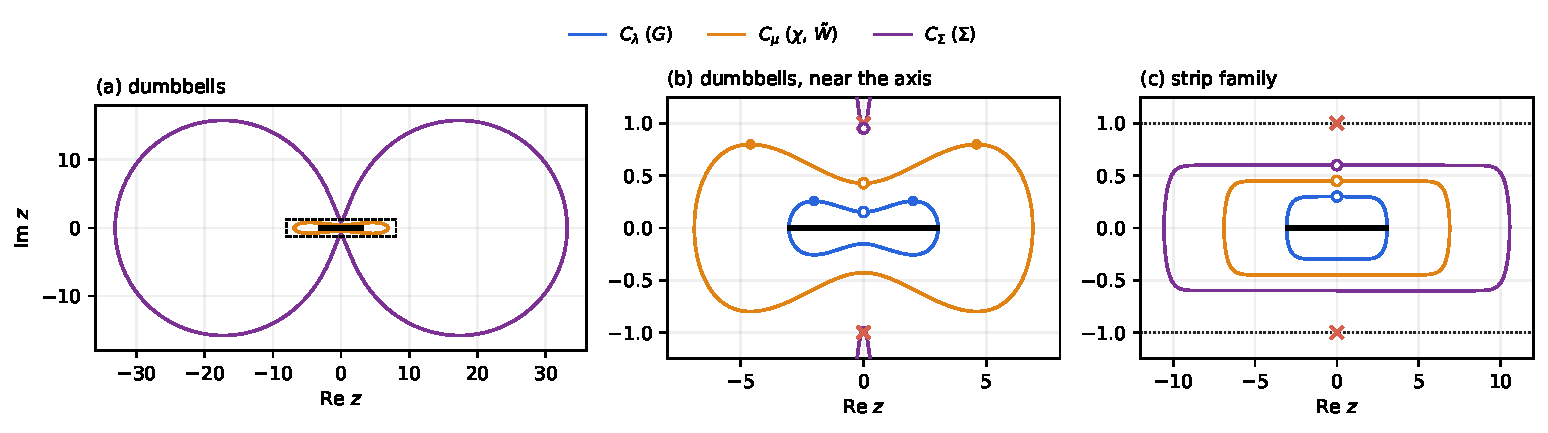
\includegraphics[width=\textwidth]{gw_chain.pdf}
  \caption{The contours of the G0W0 test chains of Table~\ref{tab:gw}: $C_\lambda$ of $G$ (blue), $C_\mu$ of $\chi$ and $\tilde W$ (orange) and $C_\Sigma$ of $\Sigma$ (purple), with the band $[-3,3]$ (black), the poles $\pm i$ of $f$ (crosses), the crossings of the imaginary axis (open circles) and, where they lie in the frame, the highest points (dots). (a) Dumbbells at the levels 0.10, 0.14 and 0.80. $C_\Sigma$ crosses the imaginary axis at 0.95 but reaches the height 15.8 and $\lvert w\rvert=33$. (b) The dashed box of (a): the heights 0.26 and 0.80 of $C_\lambda$ and $C_\mu$ lie below the crossings 0.43 and 0.95 of $C_\mu$ and $C_\Sigma$. (c) The strip family at the levels 0.30, 0.45 and 0.60, between the lines $\Imag z=\pm1$ (dotted), where every top is a crossing. Panels (b) and (c) are stretched vertically.}
  \label{fig:gw_chain}
\end{figure*}

\begin{figure}[t]
  \centering
  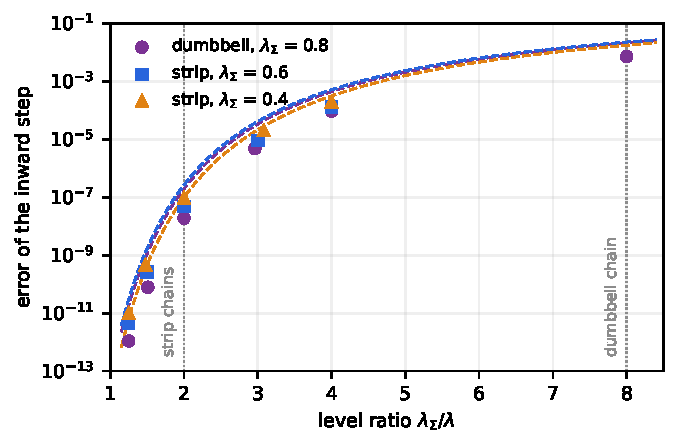
\includegraphics[width=\columnwidth]{gw_inward.pdf}
  \caption{The error of the inward step against the level ratio $\lambda_\Sigma/\lambda$, for $\Sigma$ on the contours $C_\Sigma$ of Table~\ref{tab:gw} (symbols), and the rule \eqref{eq:inward} with the forward errors of the three chains (dashed). The dumbbell chain needs the ratio 8, where the step gives $7\times10^{-3}$; the strip chains need 2, where it gives $5\times10^{-8}$ and $9\times10^{-8}$.}
  \label{fig:gw_inward}
\end{figure}

Screening and Dyson's equation are reciprocals of a train $D$ over the points of a contour and the momenta, $D=1-v_Q\Pi_Q$ and $D=z-\varepsilon_q-\Sigma_q(z)$. The Newton iteration $x\leftarrow x(2-Dx)$ squares the residual $1-Dx$ at every step, so it converges from any start with $\lvert1-Dx_0\rvert<1$ at all points. The start $x_0=D^*/\max\lvert D\rvert^2$ satisfies this, and the number of iterations grows like the logarithm of $\max\lvert D\rvert/\min\lvert D\rvert$. Cross interpolation of $1/D$ through the point evaluation of the train needs no iterations. The zeros of $D$ lie on the real axis, at the poles of $W$ and the quasiparticle poles of $G$, so $1/D$ is analytic in the same region as $D$, and its bonds stay close to those of $D$. The reciprocal fails when $D$ has zeros near the contour, which happens for an attractive $v_Q$, where $1-v_Q\Pi_Q(0)$ can vanish, or when $W$ has poles outside the chosen segment; both show up in $\min\lvert D\rvert$ on the contour and in the sum rule of $\tilde W_Q$.

The fixed-point iterations $W\leftarrow v+v\Pi W$ and $G\leftarrow G_0+G_0\Sigma G$ use only products as well, and the series $W=v+v\Pi v+\ldots$ is the first of them. Pointwise on the contour, $x\leftarrow a+bx$ converges to $a/(1-b)$ only where $\lvert b\rvert<1$, and its damped form $x\leftarrow(1-\alpha_{\rm d})x+\alpha_{\rm d}(a+bx)$ only where $\lvert1-\alpha_{\rm d}(1-b)\rvert<1$, which for a small damping $\alpha_{\rm d}$ requires $\Real b<1$ and takes about $2/[\alpha_{\rm d}\min\lvert1-b\rvert]$ steps. Newton converges for every $D$ without zeros on the contour. The iteration of the loop itself, $G\to\chi\to W\to\Sigma\to G$, has no such alternative and is damped as in any GW code.

\subsection{Tests and the order of the work}
\label{sec:gw_tests}

\begin{table*}[t]
\caption{The G0W0 self-energy of the test model at all points of $C_\Sigma$, compared with its closed form. The chain of dumbbells uses the fermionic family $(3,\pi)$ for $G_0$, the bosonic family $(6.72,\pi/2)$ for $\chi$ and $\tilde W$, and the fermionic family $(10.22,\pi)$ for $\Sigma$; the strip chains use the strip family on the same segments with $\beta=\pi$ throughout. The margins are $p(C_\mu)-H(C_\lambda)$ and $p(C_\Sigma)-\max[H(C_\lambda),H(C_\mu)]$, and $\tilde W$ is the one computed from the bubble. The errors are the largest over all momenta and points relative to $\max\lvert\Sigma^{\rm c}\rvert$; the inward step brings $\Sigma$ from $C_\Sigma$ to the level of $G$ within the family of $\Sigma$.}
\label{tab:gw}
\centering\small
\setlength{\tabcolsep}{6pt}
\begin{tabular}{@{}lcccccc@{}}
\toprule
chain & levels of $G$, $\chi$, $\Sigma$ & margins & time points & error & without $-\tilde W_Q(0)/\beta$ & inward step \\
\midrule
dumbbells & 0.10, 0.14, 0.80 & 0.17, 0.15 & 4352 & $6.3\times10^{-14}$ & 0.64 & $7.2\times10^{-3}$ \\
strip & 0.30, 0.45, 0.60 & 0.15, 0.15 & 9024 & $7.3\times10^{-14}$ & 0.20 & $4.8\times10^{-8}$ \\
strip & 0.20, 0.30, 0.40 & 0.10, 0.10 & 12096 & $1.3\times10^{-14}$ & 0.18 & $9.4\times10^{-8}$ \\
\bottomrule
\end{tabular}
\end{table*}

Dense tests on the chain \eqref{eq:model} with $E=3$, $\beta=\pi$, $N_q=64$ and the interaction $v_Q=U+2U_1\cos Q$, $U=2$, $U_1=0.5$, confirm the pieces. The zeros of $1-v_Q\Pi_Q$ lie up to $\Omega_W=6.22$, just above the continuum edge $2E$, and the families are built on $[-3,3]$ for $G_0$, $[-6.72,6.72]$ for $\chi$ and $\tilde W$, and $[-10.22,10.22]$ for $\Sigma$. The closed form of G0W0 for this model, a sum over the poles of $\tilde W$ with the static terms, agrees with the direct Matsubara sum \eqref{eq:sigma_def} to ten digits, and Table~\ref{tab:gw} compares the self-energy from \eqref{eq:sigma_time} with it, for a chain of dumbbells and for two chains of the strip family, whose contours Fig.~\ref{fig:gw_chain} shows. The self-energy is accurate to $10^{-13}$ in all three chains, its values at the Matsubara frequencies obtained from $C_\Sigma$ by the exterior Cauchy formula agree with the closed form to $2\times10^{-15}$, and without the static term the error is 18 to 64\,\%. The bubble and $\tilde W$ on $C_\mu$ are accurate to $10^{-13}$, and the density after Dyson's equation agrees with the Matsubara sum to $2\times10^{-15}$. The inward step follows \eqref{eq:inward} to within a factor of 2 above and 20 below (Fig.~\ref{fig:gw_inward}): from level 0.8 to 0.1 of the dumbbell chain it gives $7\times10^{-3}$, while from 0.6 to 0.3 of the first strip chain it gives $5\times10^{-8}$. The Newton reciprocals converge in 9 to 16 iterations, with $\max\lvert D\rvert/\min\lvert D\rvert$ from 3 to 5 for the screening and from 23 to 37 for Dyson's equation. The fixed-point iterations do not converge on these contours (Table~\ref{tab:iteration}): $\max\lvert v\Pi\rvert$ is 1.16 and 1.65 on $C_\mu$, and $\max\lvert G_0\Sigma\rvert$ is 1.05 and 1.83 on $C_\Sigma$; damping makes them converge in 117 to 2633 steps, against 9 to 16 for Newton. On the contour of $G_0$ at the level of $G$, close to the band edges, $\max\lvert G_0\Sigma\rvert$ reaches 14.8 and 38, where $G_0\Sigma$ is real and damping fails as well, and Newton needs 16 and 23 steps; on the shared family of $G$ and $\Sigma$ at level 0.3 it is 3.5. On the first strip chain the widest bond at $10^{-10}$ is 62 for $\Pi$ and for $\tilde W$, 63 for $\Sigma$ and 74 for $G$.

\begin{table*}[t]
\caption{Fixed-point iteration against Newton for screening and Dyson's equation on the chains of Table~\ref{tab:gw}, at the target $10^{-12}$. For screening $b=v_Q\Pi_Q$ on $C_\mu$ ($\max\Real b$ is 0.81 and 0.46, $\min\lvert1-b\rvert$ 0.49 and 0.60), for Dyson's equation $b=G_0\Sigma$ with the full self-energy on $C_\Sigma$, and on the contour $C_\lambda$ of $G_0$ at the level of $G$. The damped iteration is given with its best damping $\alpha_{\rm d}$; a Newton step costs two products, a fixed-point step one.}
\label{tab:iteration}
\centering\small
\setlength{\tabcolsep}{5pt}
\begin{tabular}{@{}lcccccccc@{}}
\toprule
 & \multicolumn{3}{c}{screening on $C_\mu$} & \multicolumn{3}{c}{Dyson on $C_\Sigma$} & \multicolumn{2}{c}{Dyson on $C_\lambda$} \\
chain & $\max\lvert v\Pi\rvert$ & damped & Newton & $\max\lvert G_0\Sigma\rvert$ & damped & Newton & $\max\lvert G_0\Sigma\rvert$ & Newton \\
\midrule
strip & 1.65 & 2090 ($\alpha_{\rm d}=0.3$) & 10 & 1.83 & 2633 ($\alpha_{\rm d}=0.1$) & 14 & 14.8 & 16 \\
dumbbells & 1.16 & 118 ($\alpha_{\rm d}=0.5$) & 9 & 1.05 & 117 ($\alpha_{\rm d}=0.5$) & 16 & 38.0 & 23 \\
\bottomrule
\end{tabular}
\end{table*}

The pieces can be built in the following order, each with its test.
\begin{enumerate}
  \item A dense contour GW at $N_q$ up to $10^4$, against a Matsubara GW code, before any train, and a measurement of the bonds in three dimensions before a train loop.
  \item The geometry for general $E$ and $\beta$: the dumbbell and strip families, their heights, crossings and tips, and the choice of levels. Test: the node sum of $1/(z-a)$, the symmetries and the decay of the modes.
  \item The self-energy network, dense and then as trains, reusing the bubble network: the two leaves per input, the convolution adder, the Laplace train over eight directions, the static term and the gauge. Test: the closed-form G0W0 to $10^{-13}$ and the Matsubara values by the exterior Cauchy formula. In train form the time leg is compressed to the rank of the leaves, so the network becomes the Tucker network of Appendix~\ref{app:cauchy} with the kernel \eqref{eq:kernel_time} at the tolerance of the loop; the diagonal core serves the dense tests.
  \item Screening, Dyson's equation, exchange and chemical potential as trains, by Newton or cross interpolation. Test: the bonds of the reciprocals, their pointwise accuracy and the sum rule of $\tilde W$.
  \item G0W0 at $N_q=1024$ against a Matsubara GW code: $\Sigma(i\omega_n)$, the density, the energies, and the spectral function of $\Sigma$ at the resolution set by $p(C_\Sigma)$.
  \item GW0 with the inward step on the strip family at the level ratio 2: $\Sigma$ brought to the level of $G$ on the modes $n\le\ln(1/\varepsilon_{\rm fwd})/(\alpha\lambda_\Sigma)$, Dyson's equation there, and iteration. Test: a Matsubara GW0 code at the same $\beta$, and the convergence of $\rho$ and of $\Sigma(i\omega_n)$. The accuracy of the inward step and its accumulation over the iterations are the main risk.
  \item scGW: the bubble from the dressed $G$, the support $E_G$ checked by the tail of the modes, and the poles of $W$ tracked by the sum rule of $\tilde W$. Test: a Matsubara scGW code, the particle number and the f-sum rule.
\end{enumerate}
The tests suggest the following choices.
\begin{enumerate}
  \item Use the strip family for the iterated schemes, and the dumbbells for the bubble and for G0W0, where the forward steps suffice.
  \item For the bosonic dumbbells use $\beta/2$, the doubled family of Sec.~\ref{sec:contour}, whose ratio $H/p$ on $[-6,6]$ at level 0.2 is 1.7, against 3.2 at $\beta$; for the strip family use $\beta$.
  \item Bring $\Sigma$ inward, not $G$: $\Sigma$ is smoother, and Dyson's equation at the lower level is pointwise.
  \item Do not compress inside the loop. The inward step needs the forward accuracy of the diagonal core, which a Tucker core does not reach.
  \item Keep the static terms of the finite lattice, at $Q=0$ and from degenerate pairs; the node sums include them.
  \item Heights scale like $1/\beta$ while the frequencies do not, so the time legs and the ranks grow like $\beta$. Test $\beta=2\pi$ and $4\pi$ in step 5, before the loop.
  \item Fix $E_G$ at the start with a padded segment, and widen it only when the tail of the modes exceeds the tolerance.
  \item Use margins of about 0.15, eight directions and a gauge that shares the growth between the leaves and the Laplace train.
  \item Solve screening and Dyson's equation by Newton or by cross interpolation, not by fixed-point iteration, and keep iteration for the loop.
  \item Run the loop at the lowest level its margins allow, since the continuation to the real axis (Sec.~\ref{sec:gw_continuation}) reaches the width $\eta$ with the accuracy $\varepsilon_{\rm fwd}^{\lambda'/\lambda}$.
\end{enumerate}

\subsection{Bonds, memory and cost}
\label{sec:gw_cost}

\begin{table*}[t]
\caption{Bonds and stored numbers of the trains of the GW loop at $10^{-10}$, for the chain of Sec.~\ref{sec:gw_tests} with $N_q=1024$ and for the square lattice $\varepsilon_k=-2(\cos k_x+\cos k_y)$ with $\beta=\pi$ and $v_Q=2+\cos Q_x+\cos Q_y$, on the strip chain at the levels 0.3 ($C_\lambda$), 0.45 ($C_\mu$) and 0.6 ($C_\Sigma$). The trains carry the bits of the contour index first, least significant first, and then the momentum bits. Bonds are given at $10^{-10}$ and $10^{-6}$; the stored numbers at $10^{-10}$ are compared with the dense arrays.}
\label{tab:bonds}
\centering\small
\setlength{\tabcolsep}{5pt}
\begin{tabular}{@{}lcccccc@{}}
\toprule
 & \multicolumn{2}{c}{chain, $N_q=1024$} & \multicolumn{2}{c}{square, $32\times32$} & \multicolumn{2}{c}{square, $64\times64$} \\
object & bonds & stored, dense & bonds & stored, dense & bonds & stored, dense \\
\midrule
$G_0$ on $C_\lambda$ & 176, 109 & $1.8\times10^5$, $5.2\times10^5$ & 220, 196 & $1.9\times10^5$, $5.2\times10^5$ & 527, 382 & $1.1\times10^6$, $2.1\times10^6$ \\
$\chi$ on $C_\mu$ & 132, 78 & $9.7\times10^4$, $5.2\times10^5$ & 220, 139 & $2.0\times10^5$, $5.2\times10^5$ & 431, 249 & $6.5\times10^5$, $2.1\times10^6$ \\
$\tilde W$ on $C_\mu$ & 162, 99 & $1.3\times10^5$, $5.2\times10^5$ & 220, 136 & $2.0\times10^5$, $5.2\times10^5$ & 432, 256 & $6.6\times10^5$, $2.1\times10^6$ \\
$\Sigma$ on $C_\Sigma$ & 99, 56 & $6.9\times10^4$, $1.0\times10^6$ & 223, 175 & $2.2\times10^5$, $1.0\times10^6$ & 525, 308 & $1.1\times10^6$, $4.2\times10^6$ \\
$G$ on $C_\Sigma$ & 116, 67 & $1.0\times10^5$, $1.0\times10^6$ & 223, 188 & $2.3\times10^5$, $1.0\times10^6$ & 527, 315 & $1.1\times10^6$, $4.2\times10^6$ \\
$\Sigma$ at level 0.3 & 182, 102 & $2.2\times10^5$, $1.0\times10^6$ & & & & \\
$G$ at level 0.3 & 253, 122 & $4.3\times10^5$, $1.0\times10^6$ & & & & \\
\bottomrule
\end{tabular}
\end{table*}

The bonds of a train on a contour are set by the height of the contour. A contour at height $\eta$ sees the spectrum with the width $\eta$, and the rank of $G$ over (points, momenta) is the number of energies resolved, about the bandwidth over $\eta$ times $\ln(1/\varepsilon)$. On the strip family of the chain the rank of $G_0$ at $10^{-10}$ is 443, 251, 168, 102, 73 and 57 at the levels 0.1, 0.2, 0.3, 0.5, 0.7 and 0.9, which at $\beta=\pi$ are also the heights, and at level 0.3 it is 125, 168 and 168 for $N_q=256$, 1024 and 4096; it saturates once the lattice resolves the width. On the dumbbell at level 0.2, with the crossing 0.30 and the top 0.52, it is 118. The bonds of the loop are therefore those of its lowest contour, the one of $G$, and they grow like $\beta$ at a fixed level. In two dimensions the rank over (points, momenta) saturates as well, 141 and 212 at level 0.3 for $32\times32$ and $64\times64$, but the bonds inside the momentum bits do not, and the train of $G_0$ at $64\times64$ stores half of the dense array (Table~\ref{tab:bonds}).

A zip-up costs about $4Ld^2\chi^4$ operations and a Newton product with the truncation of the zip-up about $2L\chi^5$. With $\chi=176$ and $L=19$ the ten zip-ups of a GW0 iteration cost $3\times10^{12}$ operations, and the thirty Newton products of the reciprocals $2\times10^{14}$; cross interpolation of the reciprocals, at $O(L\chi^3)$ per sweep, costs far less. The best dense scheme works in imaginary time with the discrete Lehmann representation, with about $N_\tau=100$ times at $\beta E=10$ and $10^{-10}$ and every product pointwise after an FFT in momentum. It costs about $10N_qN_\tau(\log_2N_q+N_\tau)$ operations per iteration, $10^8$ at $N_q=1024$, $3\times10^{10}$ at $64^3$ and $2\times10^{12}$ at $256^3$, and stores $N_qN_\tau$ numbers, 1.6\,MB, 420\,MB and 27\,GB. The trains therefore win in memory above $N_q\approx10^4$, where their bonds have saturated, which holds in one dimension and not yet at $64\times64$ in two. In time they win above $N_q\approx3\times10^7$, about $300^3$ momenta, with cross interpolation, and above $10^9$ with Newton, provided the bonds stay near 200 in three dimensions, which remains to be checked. On the test lattices the dense scheme is faster by four to six orders of magnitude, and what the contours give there is the analytic structure: the Matsubara values by contraction, the spectral function at the resolution of the contour, and its continuation.

\subsection{Continuation to the real axis}
\label{sec:gw_continuation}

\begin{table}[t]
\caption{Continuation of the G0W0 Green function of the test model to the lines $\Imag z=\eta$, on the strip family of $\Sigma$ with $N=8192$ nodes and data with a relative noise of $10^{-13}$: the error of the spectral function over the band relative to its maximum, for $G$ continued by the multiplier, for $\Sigma$ continued and Dyson's equation solved on the lower contour, for the rule \eqref{eq:inward}, and for a rational fit (AAA) of the samples, given as the range over five momenta.}
\label{tab:continuation}
\centering\footnotesize
\setlength{\tabcolsep}{3pt}
\begin{tabular}{@{}lcccc@{}}
\toprule
$\eta$ & 0.2 & 0.1 & 0.05 & 0.02 \\
\midrule
level 0.3, $G$ & $7.6\times10^{-10}$ & $2.4\times10^{-5}$ & $4.5\times10^{-3}$ & 0.11 \\
\quad $\Sigma$, Dyson & $4.2\times10^{-9}$ & $2.3\times10^{-4}$ & $1.8\times10^{-2}$ & 0.47 \\
\quad rule & $2.2\times10^{-9}$ & $4.6\times10^{-5}$ & $6.8\times10^{-3}$ & 0.14 \\
\quad AAA & & & 0.003 to 0.016 & 0.01 to 0.27 \\
level 0.9, $G$ & $6.9\times10^{-4}$ & $2.6\times10^{-2}$ & 0.16 & 0.47 \\
\quad rule & $1.3\times10^{-3}$ & $3.6\times10^{-2}$ & 0.19 & 0.51 \\
\bottomrule
\end{tabular}
\end{table}

On the strip family the contour at level $\lambda'$ runs along the line $\Imag z=\lambda'\pi/\beta$ over the band, apart from its tips. The train of $G$ brought to that level by the multiplier \eqref{eq:multiplier}, with the modes above $\ln(1/\varepsilon_{\rm fwd})/(\alpha\lambda)$ removed, is therefore $G(\varepsilon+i\eta)$ with $\eta=\lambda'\pi/\beta$, the spectral function with the Lorentzian width $\eta$, to the accuracy $\varepsilon_{\rm fwd}^{\lambda'/\lambda}$ of \eqref{eq:inward}. In train form these are the operations of the inward step: the DFT, the multiplier, the window and the DFT back. For the G0W0 Green function of the test model, from level 0.3 and $\varepsilon_{\rm fwd}=10^{-13}$, the widths 0.2, 0.1 and 0.05 are reached to $8\times10^{-10}$, $2\times10^{-5}$ and $5\times10^{-3}$ (Table~\ref{tab:continuation}). Continuing $\Sigma$ and solving Dyson's equation on the lower contour is worse by a factor 4 to 10, because Dyson's equation there amplifies the error of $\Sigma$ by $\lvert G\rvert^2$. From level 0.9, close to the height of the first Matsubara frequency, the exponent is $\lambda'/0.9$ instead of $\lambda'/0.3$, and the width 0.1 is already lost. The level $\lambda'$ needs the modes up to $\ln(1/\varepsilon)/(\alpha\lambda')$ for the accuracy $\varepsilon$, about 770 at $\lambda'=0.05$ for $5\times10^{-3}$, so the contour of $G$ must carry two to four more bits than the loop needs: with $N=1024$ nodes the errors from level 0.3 are $2\times10^{-7}$, $5\times10^{-4}$, $2\times10^{-2}$ and 0.2. A rational fit of the samples on the contour (AAA, 120 support points per momentum) gives comparable errors at $\eta=0.05$ and smaller ones for four of five momenta at $\eta=0.02$; it runs on slices of the train, one momentum at a time, and fails at $\eta=0$, where the exact spectrum of the finite lattice is a set of poles. The width reachable at a given accuracy $\varepsilon$ is $\eta=(\lambda\pi/\beta)\ln(1/\varepsilon)/\ln(1/\varepsilon_{\rm fwd})$, so the loop should run at the lowest level its margins allow.

\appendix

\section{The Cauchy route}
\label{app:cauchy}

In this appendix $G_{q\pm Q}$ at the shifted points $z\pm w$ is obtained from its values on $C_\lambda$ with Cauchy's formula, instead of the time representation of Sec.~\ref{sec:time}. This route covers all of $C_\mu$, its tips included, when the shifted points lie outside $C_\lambda$, that is $\lambda'_{\min}>\lambda$ in \eqref{eq:lammin}. Appendices~\ref{sec:qtt} to~\ref{sec:accuracy} build its tensor network and test it. Appendix~\ref{app:kernel_time} builds its kernel from the time route, which needs only $\lambda<\Lambda(\mu,\beta)$.

Formula \eqref{eq:contour_w} needs $G_{q\pm Q}$ at the shifted points $z\pm w$, off the contour, while the data are the values of $G$ on the dumbbell $C_\lambda$, and the method evaluates $G$ only there. Cauchy's formula, the first equality in \eqref{eq:lehmann}, gives $G(x)$ at every $x$ outside $C_\lambda$. For $x$ \emph{inside} $C_\lambda$ the same integral gives $0$ instead of $G(x)$: then $s\mapsto G(s)/(x-s)$ is analytic outside $C_\lambda$ and $O(s^{-2})$, so its integral over $C_\lambda$ equals its integral over $C_R$, which vanishes. With $x=z\pm w$ in \eqref{eq:contour_w}, the bubble becomes a double integral over the dumbbell, in which $G$ enters only on $C_\lambda$:
\begin{equation}
  \begin{aligned}
  \chi_Q(w)={}&\frac1{N_q}\sum_q\frac1{(2\pi i)^2}\oint_{C_\lambda}dz\oint_{C_\lambda}ds\;f(z)\,G_q(z)\\
  &\times\left[\frac{G_{q+Q}(s)}{z-s+w}+\frac{G_{q-Q}(s)}{z-s-w}\right].
  \end{aligned}
  \label{eq:double_contour}
\end{equation}

\subsection{The exterior-Cauchy form}
\label{app:ext_cauchy}

The rule $\frac1{2\pi i}\oint_{C_\lambda}F\,dz\approx\sum_md_m\,F(z_m)$ of Sec.~\ref{sec:quadrature} turns the Cauchy formula in \eqref{eq:lehmann} into a sum over the nodes,
\begin{equation}
  G(x)=\sum_{m=0}^{N-1}d_m\,\frac{G(z_m)}{x-z_m}\qquad(x\ \text{outside }C_\lambda),
  \label{eq:ext_cauchy}
\end{equation}
up to the trapezoidal error. The two rules applied to \eqref{eq:double_contour}, $c_j$ for the integral over $z$ and $d_m$ for the integral over $s$, give the \emph{exterior-Cauchy form} of the bubble,
\begin{equation}
\begin{aligned}
\chi_Q(w_k)={}&\frac1{N_q}\sum_q\sum_{j,m}c_j\,G_q(z_j)\,d_m\\
&\times\left[\frac{G_{q+Q}(z_m)}{z_j-z_m+w_k}+\frac{G_{q-Q}(z_m)}{z_j-z_m-w_k}\right].
\end{aligned}
\label{eq:cauchy_form}
\end{equation}

\subsection{Fourier modes and the kernel}
\label{sec:modes}

The output is expanded on $C_\mu$ in the same way as $G$ in \eqref{eq:ghat},
\begin{equation}
  \begin{aligned}
  \chi_Q(w_k)&=\sum_\ell\hat\chi_{Q,\ell}\,e^{i\pi\ell\phi_k/4},\\
  \hat\chi_{Q,\ell}&=\frac1N\sum_{k=0}^{N-1}\chi_Q(w_k)\,e^{-i\pi\ell\phi_k/4}.
  \end{aligned}
  \label{eq:chihat}
\end{equation}

Insert \eqref{eq:ghat} for $G_q(z_j)$ (index $n'$) and for $G_{q\pm Q}(z_m)$ (index $n$) into \eqref{eq:cauchy_form}. The momentum average factorizes from the geometry:
\begin{equation}
  \begin{aligned}
  \chi_Q(w_k)&=\sum_{n',n}\Big[P^+_Q(n',n)\,K_{n'n}(w_k)\\
  &\qquad\quad+P^-_Q(n',n)\,K_{n'n}(-w_k)\Big],\\
  K_{n'n}(w)&=\sum_{j,m}c_j\,d_m\,\frac{e^{i\pi(n'\phi_j+n\phi_m)/4}}{z_j-z_m+w},\\
  P^\pm_Q(n',n)&=\frac1{N_q}\sum_q\hat g_{q,n'}\hat g_{q\pm Q,n},
  \end{aligned}
\end{equation}
with the kernel $K_{n'n}$ and the momentum correlations $P^\pm_Q$. Since $\phi_{k+N/2}=\phi_k+4$ and $\omega(\zeta+4)=-\omega(\zeta)$ \eqref{eq:symmetries}, $-w_k=w_{k+N/2}$, so the second term is the first kernel read at $k+N/2$. Project on the output modes with \eqref{eq:chihat}; for the second term substitute $k'=k+N/2$ and use $\phi_k=\phi_{k'}-4$, which produces $e^{i\pi\ell}=(-1)^\ell$:
\begin{equation}
  \begin{aligned}
  \hat\chi_{Q,\ell}&=\sum_{n',n}\widehat K_{n'n\ell}\big[P^+_Q(n',n)+(-1)^\ell P^-_Q(n',n)\big],\\
  P^\pm_Q(n',n)&=\frac1{N_q}\sum_q\hat g_{q,n'}\,\hat g_{q\pm Q,n},
  \end{aligned}
  \label{eq:modes_bubble}
\end{equation}
\begin{equation}
\begin{aligned}
\widehat K_{n'n\ell}={}&\frac1N\sum_ke^{-i\pi\ell\phi_k/4}\\
&\times\sum_{j,m}c_j\,d_m\,\frac{e^{i\pi(n'\phi_j+n\phi_m)/4}}{z_j-z_m+w_k}.
\end{aligned}
\label{eq:kernel}
\end{equation}
This is the exterior-Cauchy form \eqref{eq:cauchy_form}, where the kernel depends only on the two dumbbells and on $\beta$ (through $c_j$); all of $G$, model and momentum, is in $P^\pm_Q$. For each $k$ the inner double sum is a two-dimensional FFT over $(j,m)$ of the array $c_jd_m/(z_j-z_m+w_k)$, and the outer sum is an FFT over $k$. In exact arithmetic the sums in \eqref{eq:modes_bubble} run over all $N$ values of $n'$, $n$ and $\ell$. In practice only a window of each index matters, because the coefficients of $G$ and of $\chi$ decay exponentially (Appendix~\ref{sec:decay}).

\subsection{Compressing the kernel}
\label{sec:tucker}

The kernel \eqref{eq:kernel} is compressed into Tucker form by a truncated higher-order SVD (HOSVD). For a tensor $T_{n'n\ell}$ let $T_{(i)}$ be its mode-$i$ unfolding (the matrix with the $i$-th index as rows and the other two, combined, as columns). The HOSVD takes for $U^{(i)}$ the leading left singular vectors of $T_{(i)}$ and forms the core $C=T\times_1U^{(1)\dagger}\times_2U^{(2)\dagger}\times_3U^{(3)\dagger}$, i.e.
\begin{equation}
  \begin{aligned}
  C_{abc}&=\sum_{n'n\ell}T_{n'n\ell}\,\overline{U^{(1)}_{n'a}}\,\overline{U^{(2)}_{nb}}\,\overline{U^{(3)}_{\ell c}},\\
  T_{n'n\ell}&\approx\sum_{a=1}^{r_1}\sum_{b=1}^{r_2}\sum_{c=1}^{r_3}C_{abc}\,U^{(1)}_{n'a}\,U^{(2)}_{nb}\,U^{(3)}_{\ell c}.
  \end{aligned}
  \label{eq:tucker}
\end{equation}
Each rank $r_i$ is the smallest with $\sum_{s>r_i}(\sigma^{(i)}_s)^2\le\frac{\varepsilon^2}3\lVert T\rVert_F^2$, $\sigma^{(i)}_s$ the singular values of $T_{(i)}$. Since the three truncations are orthogonal projections, their errors add at most in quadrature, $\lVert T-\hat T\rVert_F^2\le\sum_i\sum_{s>r_i}(\sigma^{(i)}_s)^2\le\varepsilon^2\lVert T\rVert_F^2$, so $\varepsilon$ bounds the relative error of the compressed tensor. The result is quasi-optimal: its error is at most $\sqrt3$ times that of the best Tucker approximation with the same ranks. Applied to the weighted kernel $\widetilde K_{n'n\ell}=s_{n'}s_n\widehat K_{n'n\ell}$ of Appendix~\ref{sec:decay}, whose weights $s_n$ make a relative truncation error of $\widetilde K$ an error of the same size in $\hat\chi$,
\begin{equation}
s_{n'}\,s_n\,\widehat K_{n'n\ell}\approx\sum_{a,b,c}C_{abc}\,U^{(1)}_{n'a}\,U^{(2)}_{nb}\,U^{(3)}_{\ell c},
\label{eq:kernel_tucker}
\end{equation}
at $\varepsilon=10^{-8}$ the ranks are $(r_1,r_2,r_3)=(31,33,44)$ for $(\lambda,\mu)=(0.2,0.4)$ and $(56,60,87)$ for $(0.1,0.2)$. The core has $r_1r_2r_3=45\,012$ entries in the example.

Inserting \eqref{eq:kernel_tucker} into \eqref{eq:modes_bubble} and absorbing the weights into the leaves, $\tilde U^{(i)}_{na}=U^{(i)}_{na}/s_n$, gives the bubble in factorized form, the formula the network computes:
\begin{equation}
\begin{aligned}
A_{q,a}&=\sum_n\hat g_{q,n}\,\tilde U^{(1)}_{na},\qquad B_{q,b}=\sum_n\hat g_{q,n}\,\tilde U^{(2)}_{nb},\\
Y^\pm_c(Q)&=\frac1{N_q}\sum_q\sum_{a,b}A_{q,a}\,C_{abc}\,B_{q\pm Q,b},\\
\hat\chi_{Q,\ell}&=\sum_cU^{(3)}_{\ell c}\Big[Y^+_c(Q)+(-1)^\ell\,Y^-_c(Q)\Big],\\
\chi_Q(w_k)&=\sum_\ell\hat\chi_{Q,\ell}\,e^{i\pi\ell\phi_k/4}.
\end{aligned}
\label{eq:factorized}
\end{equation}
Per momentum the input is reduced to $r_1+r_2$ numbers; $Y^\pm$ are $r_1r_2$ cyclic correlations in $q$ contracted with the core; the output needs $r_3$ modes. Nothing in \eqref{eq:factorized} depends on $N$ except the final synthesis. For any $G$, the definition of $Y^\pm$ gives the exact identity
\begin{equation}
  Y^-_c(Q)=Y^+_c(-Q\bmod N_q),
  \label{eq:yminus_identity}
\end{equation}
since $B_{q-Q,b}=B_{q+(-Q),b}$. The branch $Y^-$ therefore follows from $Y^+$ by the reflection $Q\to-Q$, without a second contraction (Appendix~\ref{sec:contraction}), and since the reflection changes a bond by at most a factor 2, the bonds of the two branches agree within that factor. For the even band $\varepsilon_q=3\cos q$ the two branches are equal: $A_{-q,a}=A_{q,a}$ and $B_{-q,b}=B_{q,b}$, and the substitution $q\to-q$, which maps the momentum grid onto itself, gives
\begin{equation}
  \frac1{N_q}\sum_qA_{q,a}B_{q-Q,b}=\frac1{N_q}\sum_qA_{q,a}B_{q+Q,b},
  \label{eq:reflection}
\end{equation}
that is, $Y^-(Q)=Y^+(Q)$ exactly on the grid. Then $\hat\chi_{Q,\ell}=[1+(-1)^\ell]\sum_cU^{(3)}_{\ell c}Y^+_c(Q)$: the odd modes vanish, which is the evenness $\chi_Q(-w)=\chi_Q(w)$ of the bubble of an even band. Computed by two separate zip-ups, each recompressed at $10^{-9}$, the two trains differ by $\lVert Y^--Y^+\rVert/\lVert Y^+\rVert=1.6\times10^{-11}$. The network does not use this symmetry: it computes both branches, as it must for a band that is not even.

The ranks are small because $G$ and $\chi$ enter only through Cauchy transforms. Equation \eqref{eq:spectral} writes the bubble as the average of $[f(\varepsilon)-f(\varepsilon')]/(w+\varepsilon-\varepsilon')$ with the weights $A_q(\varepsilon)A_{q+Q}(\varepsilon')$: a trilinear form in $fA_q$, $A_{q+Q}$ and the output kernel $1/(w+\varepsilon-\varepsilon')$, and \eqref{eq:cauchy_form} is its discretization. The first $G$ enters only through $\sum_jc_jG_q(z_j)/(z_j-x)=\int f(\varepsilon)A_q(\varepsilon)\,d\varepsilon/(\varepsilon-x)$, the Cauchy transform of $fA_q$ at the points $x=z_m-w_k$; the second through the Cauchy transform of $A_{q\pm Q}$ at $z_j\pm w_k$; and the output is the Cauchy transform of a two-particle spectral function on $[-2E,2E]$, evaluated on $C_\mu$. So each leg of $\widetilde K$ is a Cauchy kernel $1/(x-\varepsilon)$ between a segment and a set at a positive distance from it, with $\Lambda(\mu,\beta)$ the lowest level of the cloud $[-E,E]\pm C_\mu$ (Sec.~\ref{sec:contour}):
\begin{center}\footnotesize
\setlength{\tabcolsep}{3pt}
\begin{tabular}{@{}lp{2.3cm}p{2.7cm}p{1.6cm}@{}}
\toprule
leg & \rr source segment & \rr target set & \rr lowest level of the target \\
\midrule
1 ($n'$) & \rr $[-E,E]$, weight $fA$ & \rr $[-E,E]-C_\mu$ (the ``cloud'') & \rr $\Lambda(\mu,\beta)$ \\
2 ($n$) & \rr $[-E,E]$, weight $A$ & \rr $[-E,E]+C_\mu$ (the same set) & \rr $\Lambda(\mu,\beta)$ \\
3 ($\ell$) & \rr $[-2E,2E]$ (doubled family, level 0) & \rr $C_\mu$ & \rr $\mu$ \\
\bottomrule
\end{tabular}
\end{center}
In dumbbell coordinates a Cauchy kernel from the band to a contour at level $\Lambda$ is the diagonal multiplier $e^{-\alpha\Lambda n}$ of \eqref{eq:multiplier}, so its singular values decay exponentially at the rate $\alpha\Lambda$ and its $\varepsilon$-rank is $\log(1/\varepsilon)/(\alpha\Lambda)$. The discrete Lehmann representation works the same way, with the dumbbell level in the role of $\log\Lambda_{\rm DLR}$. Measured for $\mu$ from 0.2 to 0.8, the ranks follow, within 3\,\%,
\begin{equation}
  r_3\approx0.90\,\frac{\log(1/\varepsilon)}{\alpha\mu},\qquad r_{1,2}\approx0.65\,\frac{\log(1/\varepsilon)}{\alpha\Lambda(\mu,\beta)} ;
  \label{eq:ranklaw}
\end{equation}
for $\varepsilon=10^{-8}$ this gives $42$ and $31$ at $\mu=0.4$ (measured 44 and 31), and $84$ and $53$ at $\mu=0.2$ (measured 87 and 56). The prefactors are below 1 because the HOSVD measures the error in the Frobenius norm over the whole cloud, most of which lies far above level $\Lambda$; the sup-norm version (the number of poles needed to represent a Green function on $C_\Lambda$) is $\log(1/\varepsilon)/(\alpha\Lambda)$ within 1 to 3\,\%. The ranks therefore grow like $\log(1/\varepsilon)$ (about $+9$ per two decades for $(0.2,0.4)$ and $+16$ for $(0.1,0.2)$), like $1/\mu$, and roughly linearly with $\beta$ at fixed level, because at fixed level the whole dumbbell family moves toward the real axis as $T\to0$. They do not depend on $N$ or on $\lambda$.

\subsection{The kernel from the time route}
\label{app:kernel_time}

The tensors \eqref{eq:vandermonde} give the kernel of this route in canonical form, with the time leg as its rank,
\begin{equation}
  K^{\rm t}_{n'nk}=\sum_p\varpi_p\,V^{(1)}_{n',p}\,V^{(2)}_{n,p}\,\Lambda_{p,k}.
  \label{eq:kernel_time}
\end{equation}
By \eqref{eq:time_nodes}, $X_Q(w_k)=\sum_{n',n}P^+_Q(n',n)\,K^{\rm t}_{n'nk}$, which is the first term of the bubble in Appendix~\ref{sec:modes} with $K^{\rm t}_{n'nk}$ in place of $K_{n'n}(w_k)$, and the second term is $X_{-Q}(w_{k+N/2})$, read at $k+N/2$ as there. When the copies $C_\lambda\pm w_k$ lie outside $C_\lambda$, the two kernels agree up to the quadrature errors. When they overlap $C_\lambda$, $K_{n'n}(w_k)$ no longer gives the bubble, while $K^{\rm t}$ still does for every $G$ analytic off the band, because it comes from \eqref{eq:shrink2} applied to products of exponentials. Projected on the output modes with \eqref{eq:chihat} and weighted by $s_{n'}s_n$, $K^{\rm t}$ takes the place of $\widehat K$ in \eqref{eq:kernel_tucker}, and the network of Appendices~\ref{sec:qtt} to~\ref{sec:accuracy} runs unchanged on all of $C_\mu$ whenever $\lambda<\Lambda(\mu,\beta)$.

For $N_q=64$ and $(\lambda,\mu)=(0.2,0.4)$, $K^{\rm t}$ agrees with $K_{n'n}(w_k)$ on the window of modes to $2.2\times10^{-11}$ of its largest entry, its HOSVD at $10^{-8}$ has the ranks $(31,33,44)$ of Appendix~\ref{sec:tucker}, and the network with this tree gives the bubble to $1.7\times10^{-7}$. For $(0.2,0.25)$, below $\mu_{\rm fwd}(0.2)$, the two kernels differ by $36\,\%$ of the largest entry and the tree of the Cauchy kernel gives the bubble only to $5.3\times10^{-2}$, while the tree of $K^{\rm t}$ has the ranks $(46,49,70)$ and gives $5.0\times10^{-7}$.

The canonical form also compresses the time leg of Sec.~\ref{sec:quadrature}. Let $U^{(3)}$ hold the leading left singular vectors of the unfolding of the weighted $K^{\rm t}$ over its output index $k$. Replacing $\Lambda$ by $\Lambda U^{(3)}U^{(3)\dagger}$ reduces the output leg to $r_3$ at the accuracy of the truncation: at $(0.2,0.4)$, $r_3=44$ and the error $1.6\times10^{-7}$ at $10^{-8}$, and $r_3=55$ and $2.1\times10^{-9}$ at $10^{-10}$; at $(0.2,0.25)$, 70 and $4.1\times10^{-7}$, and 88 and $7.1\times10^{-9}$. The time network can therefore trade its accuracy for the ranks of the Cauchy route.

\section{Quantics tensor trains}
\label{sec:qtt}

\begin{figure*}[tp]
  \centering
  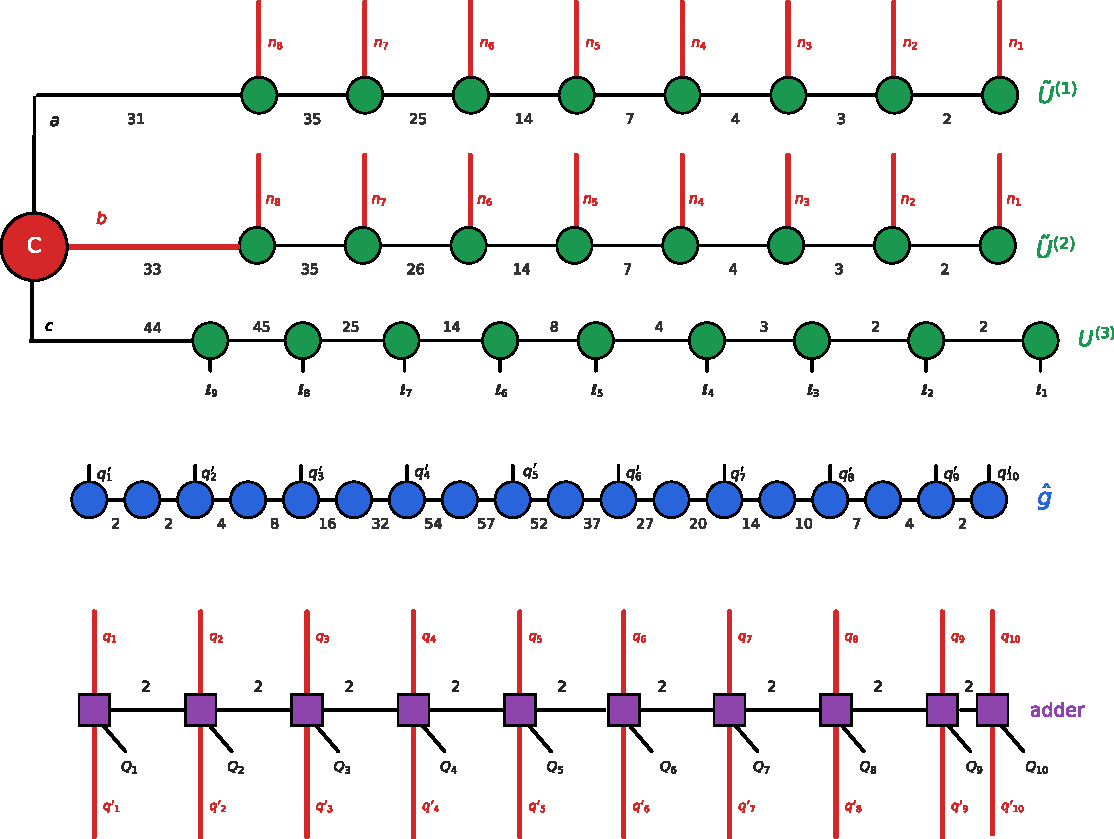
\includegraphics[width=0.82\textwidth]{ingredients_v2.pdf}
  \caption{The ingredients, with the bond dimensions of the run (tolerances in Appendix~\ref{sec:tensors}). Top: the Tucker tree of the weighted kernel, the core $C$ with the legs $a$, $b$, $c$ and the leaves $\tilde U^{(1)}$, $\tilde U^{(2)}$ over the bits $n_8\ldots n_1$ and $U^{(3)}$ over $\ell_9\ldots\ell_1$. Middle: the input $\hat g$, whose sites alternate between momentum bits and bits of $n$. Bottom: the adder, with the input legs $q_i$, $q'_i$ and the output legs $Q_i$; its bond is the carry.}
  \label{fig:ingredients}
\end{figure*}

\begin{figure*}[tp]
  \centering
  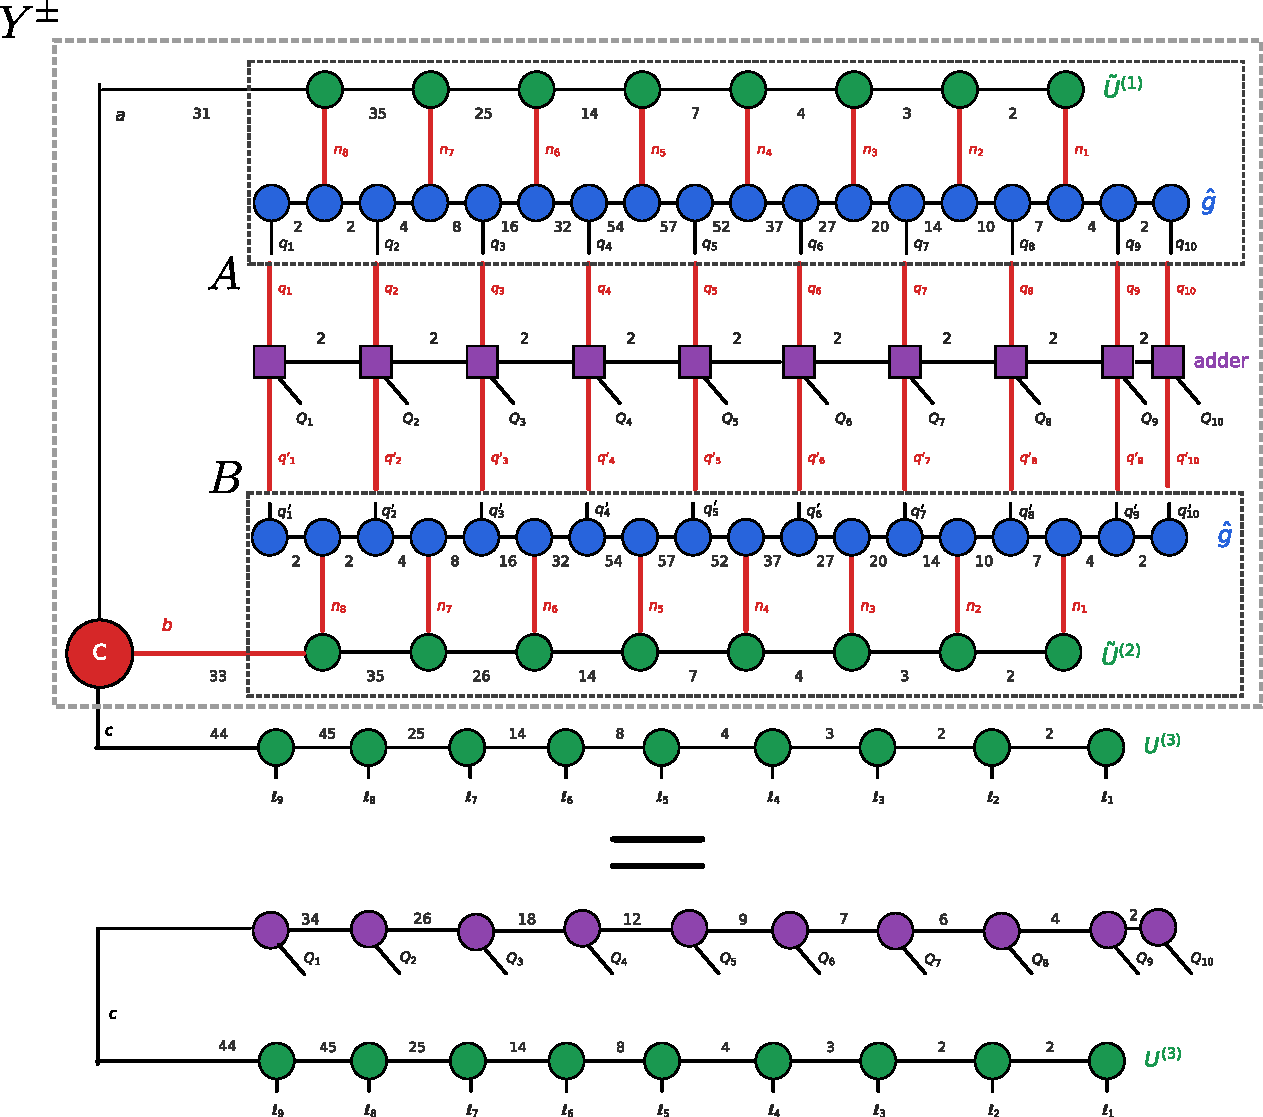
\includegraphics[width=0.84\textwidth]{bubble_tn_contraction_modified_by_me_v2.pdf}
  \caption{The network, with the bond dimensions of the run; red legs are contracted. The dashed box $A$ holds $\hat g$ and the leaf $\tilde U^{(1)}$, contracted over the legs $n_i$ in step \stp1, and the box $B$ holds $\hat g$ and $\tilde U^{(2)}$, contracted in step \stp2. The grey dashed box is the network of step \stp4, whose result is the train $Y^\pm(Q;c)$: $A$ and $B$ joined by the adder over the legs $q_i$, $q'_i$, with the core $C$ on their legs $a$ and $b$. The output leaf $U^{(3)}$ is attached through $c$. Below the equals sign is the same network after step \stp4. The drawing shows $Y^+$. For $Y^-$ the adder is replaced by the subtractor ($q'=q-Q$, bond: the borrow) and $U^{(3)}$ carries the sign $(-1)^\ell=(-1)^{\ell_9}$; the bonds are the same. By \eqref{eq:yminus_identity}, the $Y^-$ network equals the $Y^+$ network read at $-Q$.}
  \label{fig:contraction}
\end{figure*}

An index $q\in\{0,\ldots,2^R-1\}$ is written in binary,
\begin{equation}
  q=\sum_{i=1}^Rq_i\,2^{R-i},\qquad q_i\in\{0,1\},
  \label{eq:bits}
\end{equation}
with $q_1$ the most significant bit and $q_R$ the least significant one. A vector $v(q)$ of length $2^R$ is thereby a tensor $v(q_1,\ldots,q_R)$ with $R$ indices of dimension $d=2$, its \emph{quantics} form; $d$ is the \emph{physical dimension} of every site. A signed index such as a Fourier mode $n\in[-2^{R-1},2^{R-1})$ is stored in \emph{two's complement}, as the bits of $n\bmod2^R$:
\begin{equation}
  n=-n_1\,2^{R-1}+\sum_{i=2}^Rn_i\,2^{R-i},
  \label{eq:twos}
\end{equation}
so $n_1$ is the sign bit, and the nonnegative modes come first, followed by the negative ones, each $n<0$ at position $2^R+n$. This is the order in which an FFT returns its modes. ``Most significant first'' means the chain carries $q_1,q_2,\ldots,q_R$ in this order; ``least significant first'' the reverse.

A tensor train (TT, or matrix-product state, MPS) writes a tensor with $L$ indices as a product of matrices, one per index (\emph{site}),
\begin{equation}
  \begin{gathered}
  v(\sigma_1,\ldots,\sigma_L)=M^{[1]}_{\sigma_1}M^{[2]}_{\sigma_2}\cdots M^{[L]}_{\sigma_L},\\
  M^{[i]}_{\sigma_i}\in\mathbb C^{\chi_{i-1}\times\chi_i},\qquad\chi_0=\chi_L=1 .
  \end{gathered}
  \label{eq:tt}
\end{equation}
The $\chi_i$ are the \emph{bond dimensions} (``bonds''); the train stores $\sum_id\,\chi_{i-1}\chi_i$ numbers instead of $d^L$. A tensor with an additional dense index (the Tucker indices $a$, $b$, $c$ below) is a train whose first or last core carries that index, so that $\chi_0$ or $\chi_L$ equals its dimension. The smallest bond $\chi_i$ that represents the tensor exactly depends only on the tensor and the site order: it is the rank of the \emph{unfolding} matrix whose rows are indexed by $(\sigma_1,\ldots,\sigma_i)$ and whose columns by $(\sigma_{i+1},\ldots,\sigma_L)$. A matrix-product operator (MPO) is the same object for a linear map, $W(\sigma'_1\ldots\sigma'_L;\sigma_1\ldots\sigma_L)=W^{[1]}_{\sigma'_1\sigma_1}\cdots W^{[L]}_{\sigma'_L\sigma_L}$, with cores carrying an input and an output bit. Applying an MPO of bond $D_W$ to a train of bond $\chi$ gives, before any compression, a train of bond $D_W\chi$.

For a function of two variables the bit strings are concatenated, and the order matters because the bonds are ranks of unfoldings. \emph{Sequential} order puts all bits of one variable before those of the other ($n_1\ldots n_R\,q_1\ldots q_{R_q}$); \emph{interleaved} order alternates them ($q_1n_1q_2n_2\ldots$), possibly with one variable reversed ($q_1n_Rq_2n_{R-1}\ldots$). Bits that interact should sit next to each other. A smooth function of two variables is best sequential: the single matrix coupling them has low rank, and interleaving spreads it over many bonds. A Fourier-type coupling $e^{2\pi i\,nq/2^R}$ is best interleaved with one variable reversed, because the bit $q_i$ couples only to the bits $n_j$ with $i+j>R$ (Appendix~\ref{app:qft}). For this reason the input $\hat g_{q,n}$ of the method is interleaved, with $n$ least significant first, and the output $\hat\chi_{Q,\ell}$ is sequential (Appendix~\ref{sec:choices}).

The cyclic correlation $\frac1{N_q}\sum_qA_qB_{q+Q}$ over the momentum grid, $N_q=2^{R_q}$, is the contraction of $A(q)$ and $B(q')$ with the tensor $\delta_{q',\,(q+Q)\bmod N_q}$, the \emph{adder}, which is an MPO of bond dimension 2 over the bits of $q$, $q'$ and $Q$. Binary addition propagates a carry $c\in\{0,1\}$ from the least significant bit upward; the local tensor at bit $i$ is
\begin{equation}
  \begin{aligned}
  \big[W^{[i]}\big]_{c_{\rm in}c_{\rm out}}(q_i,Q_i,q'_i)={}&\delta\big(q'_i,\ q_i\oplus Q_i\oplus c_{\rm in}\big)\\
  &\times\delta\big(c_{\rm out},\ \lfloor(q_i+Q_i+c_{\rm in})/2\rfloor\big),
  \end{aligned}
  \label{eq:adder}
\end{equation}
with $\oplus$ the sum modulo 2, $c_{\rm in}=0$ at the least significant bit and the carry out of the most significant bit discarded (addition modulo $N_q$: momenta are periodic). The bond index is the carry, so the bond is exactly $D_W=2$ at every site, for any $R_q$ and with no truncation. The \emph{subtractor} $\delta_{q',\,(q-Q)\bmod N_q}$ has the same form with a borrow, $q'_i=q_i\oplus Q_i\oplus b_{\rm in}$ and $b_{\rm out}=1$ iff $q_i-Q_i-b_{\rm in}<0$; equivalently, it is the adder with the roles of $q$ and $q'$ exchanged ($q=q'+Q$). In the network (Appendix~\ref{sec:contraction}) the legs $q_i$ and $q'_i$ are contracted with the two input branches and the legs $Q_i$ remain open, so one contraction gives the correlation for all $N_q$ transfer momenta at once.

The reflection $Q\to-Q\bmod N_q$ (two's-complement negation: complement every bit, then add 1) is also an MPO of bond 2: a bitwise NOT followed by the ``$+1$'' tensor $P[c_{\rm out},{\rm out},{\rm in},c_{\rm in}]=1$ iff ${\rm out}={\rm in}\oplus c_{\rm in}$ and $c_{\rm out}={\rm in}\wedge c_{\rm in}$, with $c_{\rm in}=1$ at the least significant bit and the final carry discarded.

\begin{figure*}[tp]
  \centering
  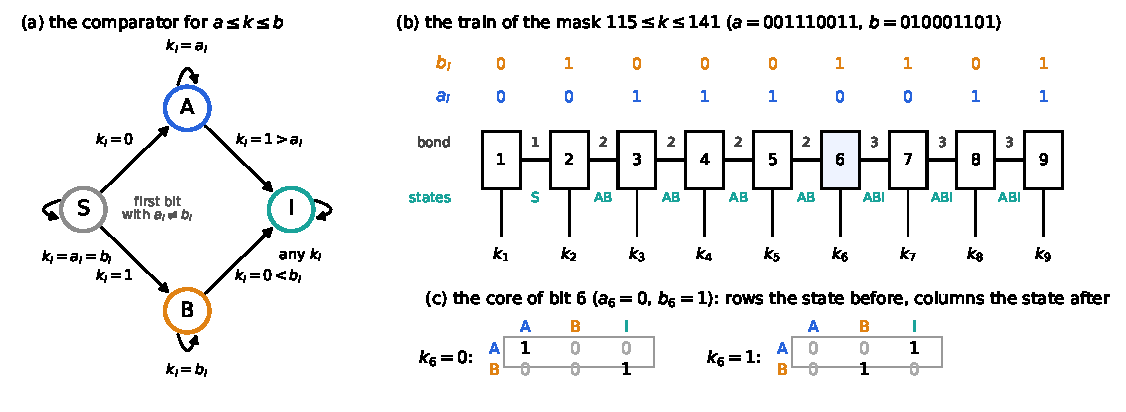
\includegraphics[width=0.95\textwidth]{mask_tt.pdf}
  \caption{The exact train of an interval mask. (a) The comparator for $a\le k\le b$, read from the most significant bit of $k$: the state records whether the bits read so far agree with those of both endpoints (S), of $a$ only (A) or of $b$ only (B), or place $k$ strictly inside the interval (I); a missing transition is a zero entry of the core. (b) The train of the mask $115\le k\le141$ of imaginary time around the right tip of $C_\mu$ (Fig.~\ref{fig:directions}), with the bits of $a$ and $b$ over the cores and the states that can occur on each bond; contracted, it reproduces the mask exactly. (c) The core of bit 6, where $a_6=0$ and $b_6=1$: two $2\times3$ tables of zeros and ones, one for each value of $k_6$.}
  \label{fig:mask_tt}
\end{figure*}

The masks $P_\gamma(w_k)$ of Sec.~\ref{sec:quadrature} are indicators of intervals of $k$, and the indicator of $a\le k\le b$ is an exact train of bond at most 3 (Fig.~\ref{fig:mask_tt}). Reading the bits of $k$ from the most significant one, the bond index records whether the bits read so far agree with those of both endpoints (S), with those of $a$ only (A) or of $b$ only (B), or already place $k$ strictly inside the interval (I). The core of bit $i$ has the entry 1 for S$\to$S when $k_i=a_i=b_i$, for S$\to$A and S$\to$B with $k_i=0$ and $k_i=1$ at the first bit where $a_i\neq b_i$, for A$\to$A when $k_i=a_i$, for A$\to$I when $k_i=1>a_i$, for B$\to$B when $k_i=b_i$, for B$\to$I when $k_i=0<b_i$, and for I$\to$I, and 0 otherwise; the train starts in S and ends in any state. At most three states are alive on a bond, since S disappears at the first difference. The mask of real time on the upper half wraps around $k=0$ and is the all-ones train minus the indicator of an interval.

A train produced by an operation (an MPO applied to a train, a sum as in Appendix~\ref{app:sum}, a contraction) in general has bonds larger than needed. A QR sweep followed by a sweep of truncated SVDs, the \emph{recompression}, brings them down to what the tolerance requires, with the error bound of TT-SVD (Appendix~\ref{app:recomp}). Every intermediate of the contraction is recompressed this way at relative tolerance $10^{-9}$.

To apply an MPO of bond $D_W$ to a train of bond $\chi$, one can form the product train (bond $D_W\chi$) and recompress it, at a cost $O(Ld\,(D_W\chi)^3)$ that is prohibitive when $D_W\chi$ reaches $10^4$ (it would be $\approx13\,800$ in step \stp4 below). The \emph{zip-up} contracts and truncates site by site in a single sweep. At site $i$ the carried matrix, whose rows are the truncated bond $\chi'_{i-1}$, is contracted with the $i$-th MPO and train cores, which produces a matrix with $d\chi'_{i-1}$ rows (the truncated bond and the output leg of site $i$) and $D_W\chi$ columns (the right bonds of the MPO and of the train); a truncated SVD factors it, $U$ becomes the finished core $i$, and $SV^\dagger$ is carried to site $i+1$. The product of bond $D_W\chi$ is never formed: the largest matrix has one side of size $d\chi'$ and the other $D_W\chi$ (the largest SVD of the run is $550\times5832$). Since the truncation at site $i$ does not yet know the sites to its right, it is slightly suboptimal; a final recompression sweep removes the excess (the two rows of bonds in Table~\ref{tab:steps}). The same scheme contracts two trains over shared physical legs: in steps \stp1 and \stp2 the leaf train is zipped along $\hat g$ over the legs $n_i$, with an SVD after every $q$ site, and in step \stp4 the adder sits between $A$ and $B'$, the legs $q_i$, $q'_i$ are summed and $Q_i$ stays open.

\section{The tensors}
\label{sec:tensors}

\begin{figure*}[tp]
  \centering
  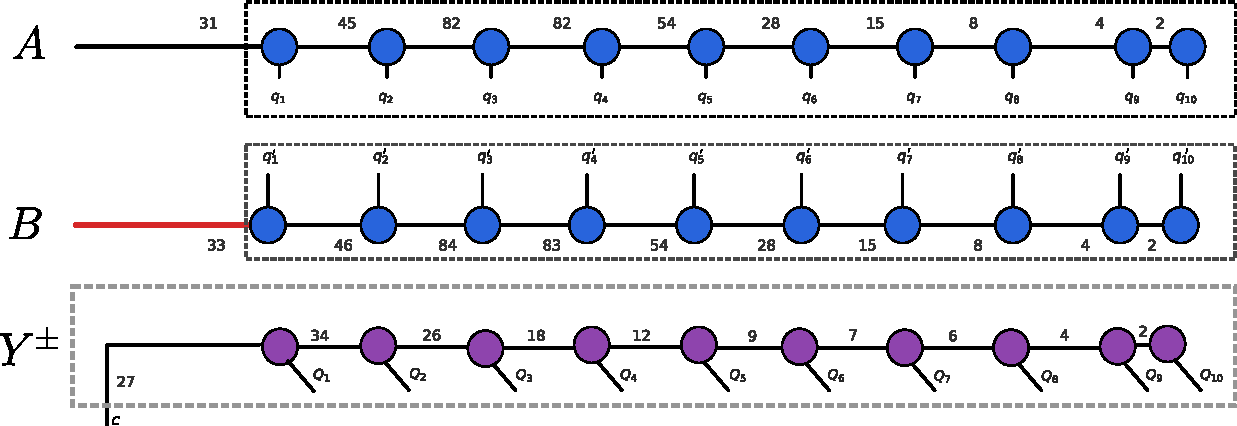
\includegraphics[width=\textwidth]{intermediate_steps_v2.pdf}
  \caption{The intermediate trains after recompression, with the bond dimensions of the run: $A(q;a)$ from step \stp1, $B(q';b)$ from step \stp2, and $Y^\pm(Q;c)$ from step \stp4, the same for both signs. Their bonds are the second rows of Table~\ref{tab:steps}.}
  \label{fig:intermediate}
\end{figure*}

\begin{table*}[t]
\caption{The contraction, step by step. For every step the bonds of the result are given before recompression (first row) and after it (second row). The first, second and fourth steps are zip-ups (Appendix~\ref{sec:qtt}), so their bonds before recompression are those left by the zip-up. In the cost column $\chi$ is the bond dimension of every train and the dimension of the Tucker legs $a$, $b$, $c$; $d=2$ is the physical dimension of the legs $q_i$, $q'_i$, $Q_i$, $n_i$, $\ell_i$, $k_i$; $D_W=2$ is the bond of the adder; $D=11$ is the bond dimension of the DFT MPO; $L$ is the number of sites.}
\label{tab:steps}
\centering\footnotesize
\setlength{\tabcolsep}{3pt}
\begin{tabular}{@{}cp{2.3cm}p{2.3cm}p{2.1cm}p{7.6cm}p{2.0cm}@{}}
\toprule
step & \rr contract & \rr over & \rr result & \rr bonds before recompression\newline $\to$ after recompression & \rr cost \\
\midrule
\stp1 & \rr $\hat g$ with $\tilde U^{(1)}$ & \rr $n_1\ldots n_8$ (zip-up, SVD after every $q$ site) & \rr $A$: $a$, $q_1\ldots q_{10}$ & \rr 31, 50, 100, 193, 293, 139, 47, 10, 4, 2\newline $\to$ 31, 45, 82, 82, 54, 28, 15, 8, 4, 2 & \rr $O(Ld^2\chi^4)$ \\
\stp2 & \rr $\hat g$ with $\tilde U^{(2)}$ & \rr $n_1\ldots n_8$ (zip-up) & \rr $B$: $b$, $q_1\ldots q_{10}$ & \rr 33, 52, 104, 196, 293, 139, 47, 10, 4, 2\newline $\to$ 33, 46, 84, 83, 54, 28, 15, 8, 4, 2 & \rr $O(Ld^2\chi^4)$ \\
\stp3 & \rr $C$ with the first site of $B$ & \rr $b$ & \rr $B'$: $(a,c)$, $q_1\ldots q_{10}$ & \rr unchanged, no recompression & \rr $O(\chi^4)$ \\
\stp4 & \rr $A$, adder (or subtractor), $B'$ & \rr $a$, $q_i$, $q'_i$ (zip-up, SVD after every site) & \rr $Y^\pm$: $c$, $Q_1\ldots Q_{10}$ & \rr 44, 88, 173, 275, 211, 101, 46, 24, 13, 7\newline $\to$ 27, 34, 26, 18, 12, 9, 7, 6, 4, 2 & \rr $O(LD_Wd^2\chi^4)$ for each sign \\
\stp5 & \rr $U^{(3)}$ with $Y^+$ and with $Y^-$, then add & \rr $c$; sign $(-1)^\ell$ on $\ell_9$ & \rr $\hat\chi$: $\ell_1\ldots\ell_9$, $Q_1\ldots Q_{10}$ & \rr 4, 4, 6, 8, 16, 28, 50, 90, 54, 68, 52, 36, 24, 18, 14, 12, 8, 4\newline $\to$ 2, 2, 2, 3, 5, 9, 16, 24, 24, 34, 26, 18, 12, 9, 7, 6, 4, 2 & \rr $O(Ld\chi^3)$ \\
\stp6 & \rr $F$ with $\hat\chi$ & \rr $\ell_1\ldots\ell_9$ & \rr $\chi$: $k_9\ldots k_1$, $Q_1\ldots Q_{10}$ & \rr 4, 8, 16, 33, 55, 72, 64, 48, 24, 34, 26, 18, 12, 9, 7, 6, 4, 2\newline $\to$ 2, 4, 7, 8, 11, 16, 20, 24, 24, 34, 26, 18, 12, 9, 7, 6, 4, 2 & \rr $O(LdD^3\chi^3)$ \\
\bottomrule
\end{tabular}

\vspace{1.5em}
\begin{minipage}{0.48\textwidth}
\caption{Error per transfer momentum $Q=2\pi m/1024$.}
\label{tab:accuracy}
\centering\small
\setlength{\tabcolsep}{6pt}
\begin{tabular}{@{}rcc@{}}
\toprule
$m$ & error & $\max_k\lvert\chi_{\rm exact}\rvert$ \\
\midrule
1 & $2\times10^{-4}$ & $3\times10^{-5}$ \\
16 & $8\times10^{-7}$ & $6\times10^{-3}$ \\
64 & $5\times10^{-8}$ & 0.05 \\
160 & $9\times10^{-9}$ & 0.10 \\
256 & $5\times10^{-9}$ & 0.13 \\
512 & $1.7\times10^{-7}$ & 0.22 \\
\bottomrule
\end{tabular}
\end{minipage}
\end{table*}

The numbers in this and the following sections are for $N_q=1024$ momenta and $N=512$ contour points, that is $R_q=10$ and $R=9$ bits, with $\lambda=0.2$ and $\mu=0.4$. In Fig.~\ref{fig:ingredients} and below, all bits are written with the most significant bit first unless stated otherwise; $n$ and $\ell$ are in two's complement, i.e.\ FFT order \eqref{eq:twos}, and bond dimensions are listed from left to right. The input $\hat g_{q,n}$ is the raw array \eqref{eq:ghat} as a train; Appendix~\ref{sec:choices} explains why the raw array is truncated and the weight $1/s_n$ is put into the leaves. The leaves are the Tucker factors of \eqref{eq:kernel_tucker} written as trains over the bits of $n$ or $\ell$, with the Tucker index attached at the least significant bit, where the leaf bonds stay below the Tucker rank. Every tensor is computed to a relative tolerance $\varepsilon$, in the sense of Appendix~\ref{sec:tucker} for the HOSVD and of Appendix~\ref{app:ttsvd} for the trains:
\begin{center}\footnotesize
\setlength{\tabcolsep}{4pt}
\begin{tabular}{@{}p{2.9cm}p{3.1cm}l@{}}
\toprule
\rr tensor & \rr computed by & $\varepsilon$ \\
\midrule
\rr Tucker tree: core $C$, factors $U^{(i)}$ & \rr HOSVD of the weighted kernel & $10^{-8}$ \\
\rr input $\hat g_{q,n}$ & \rr TT-SVD of the raw array & $10^{-6}$ \\
\rr leaves $\tilde U^{(1)}$, $\tilde U^{(2)}$, $U^{(3)}$ & \rr TT-SVD & $10^{-10}$ \\
\rr inverse DFT $F$ & \rr TT-SVD of the MPO & $10^{-12}$ \\
\rr adder, subtractor & \rr exact, bond 2 & none \\
\rr intermediates of the contraction & \rr zip-up and recompression & $10^{-9}$ \\
\bottomrule
\end{tabular}
\end{center}


\section{The contraction}
\label{sec:contraction}

Step \stp1 contracts $\hat g$ with the leaf $\tilde U^{(1)}$ over the legs $n_1\ldots n_8$, and step \stp2 contracts it with $\tilde U^{(2)}$; these are the dashed boxes $A$ and $B$ of Fig.~\ref{fig:contraction}, with the contracted legs in red. The core $C$ is then contracted with the first site of $B$ over $b$ (step \stp3), which gives $B'$. The grey dashed box is the network of step \stp4: $A$ and $B'$ joined by the adder (for $Y^+$) or the subtractor (for $Y^-$) over the legs $q_i$ and $q'_i$, with only $c$ and $Q_1\ldots Q_{10}$ left open. Its result is the train $Y^\pm(Q;c)$, drawn below the equals sign, still attached to the output leaf $U^{(3)}$ through $c$. Step \stp5 does this last contraction for both signs, with the sign $(-1)^\ell$ on $\ell_9$ for $Y^-$, and adds the two branches. Step \stp6, the inverse DFT $\ell\to k$ (Appendix~\ref{app:qft}), is not drawn. Figure~\ref{fig:intermediate} shows the recompressed trains $A$, $B$ and $Y^\pm$, and Table~\ref{tab:steps} gives the bonds and the cost of every step.

With both zip-ups of step \stp4, 29\,s each, the contraction takes about 60\,s. The largest bond after recompression is 84, in $B$; from the core on, every bond is at most 34, the bond of the result itself. Three objects are never formed: the weighted input $\hat g/s$, which is incompressible; the correlation $M(Q;a,b)$, whose leg has dimension 1023; and the uncompressed products inside the zip-ups, whose bond would reach $\approx13\,800$ in step \stp4.

The branch $Y^-$ does not need its own zip-up. By \eqref{eq:yminus_identity}, $Y^-(Q)=Y^+(-Q\bmod N_q)$: the subtractor version of Fig.~\ref{fig:contraction} is the adder version read at the reflected momentum. The reflection $Q\to-Q$ is the bitwise NOT on every $Q$ bit followed by the exact ``$+1$'' MPO of bond 2 (Appendix~\ref{sec:qtt}), applied to the train $Y^+(Q;c)$. The reflection takes 0.01\,s, and the reflected $Y^+$ agrees with $Y^-$ from the subtractor zip-up to $1.7\times10^{-10}$. We therefore recommend one zip-up for $Y^+$ (29\,s) followed by the reflection; the whole contraction then takes about 31\,s instead of 60\,s.

\section{Accuracy}
\label{sec:accuracy}

Compared with the Lindhard bubble \eqref{eq:lindhard} at all 1024 transfer momenta and all 512 points of $C_\mu$, the network gives
\begin{equation}
\max_{Q,k}\lvert\chi-\chi_{\rm exact}\rvert\Big/\max_{Q,k}\lvert\chi_{\rm exact}\rvert=1.7\times10^{-7}.
\end{equation}
Table~\ref{tab:accuracy} gives the error per transfer momentum $Q=2\pi m/1024$, $\max_k\lvert\chi-\chi_{\rm exact}\rvert/\max_k\lvert\chi_{\rm exact}\rvert$. The absolute error is about $10^{-8}$ at every $Q$; the relative error grows at small $Q$ only because $\chi_Q$ itself vanishes there. The contraction adds no error above $10^{-9}$: the MPS result and the same factors contracted densely agree to that level. The error comes from the compressions, mainly that of the kernel at $10^{-8}$; by Appendix~\ref{sec:decay}, a relative truncation of the weighted kernel is directly an error of $\hat\chi$.

\section{The Lindhard function}
\label{app:lindhard}

\begin{figure}[t]
  \centering
  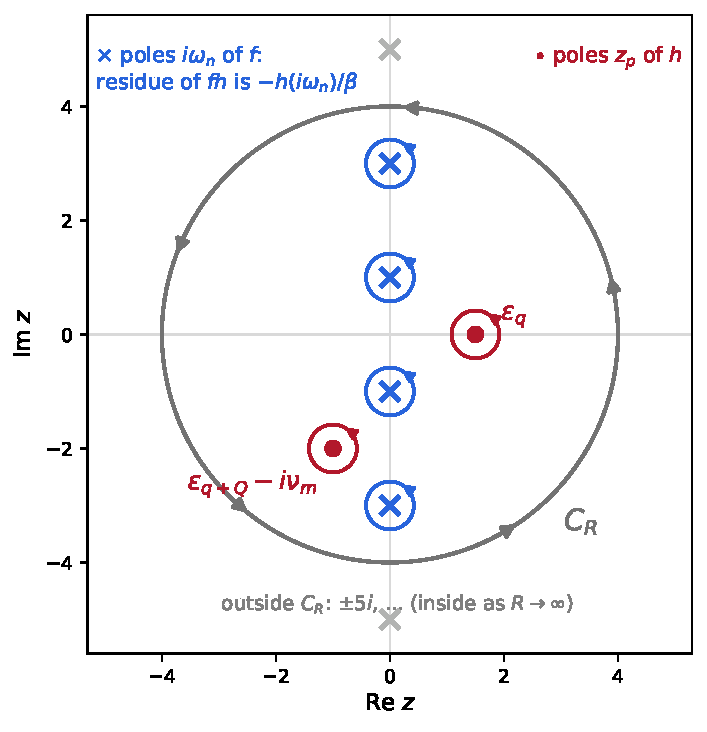
\includegraphics[width=\columnwidth]{residues_eq6.pdf}
  \caption{The residue argument behind \eqref{eq:residues_h}, for $\beta=\pi$ and the $h$ of the model with $m=1$. Crosses: the poles $i\omega_n=\pm i,\pm3i,\ldots$ of $f$, where $fh$ has the residues $-h(i\omega_n)/\beta$. Dots: the poles of $h$, $\varepsilon_q$ (here 1.5) and $\varepsilon_{q+Q}-i\nu_m$ (here $-1-2i$). The integral over the circle $C_R$ equals the sum of the integrals over the small circles, i.e.\ $2\pi i$ times all residues inside $C_R$. It tends to zero as $R\to\infty$, so the residues at the crosses and at the dots add up to zero.}
  \label{fig:residues}
\end{figure}

For the model \eqref{eq:model}, $h(z)=G_q(z)\,G_{q+Q}(z+i\nu_m)=1/[(z-\varepsilon_q)(z+i\nu_m-\varepsilon_{q+Q})]$ has only two poles, and the residues at the Matsubara frequencies in \eqref{eq:matsum_residues} can be traded for the residues at these two poles (Fig.~\ref{fig:residues}).

Let $h$ be meromorphic and $O(z^{-2})$ at infinity, with poles $z_p$ none of which is a Matsubara frequency, and let $C_R$ be the circle $\lvert z\rvert=R$, counterclockwise, with $R$ an even multiple of $\pi/\beta$, halfway between two poles of $f$. By the residue theorem, $\frac1{2\pi i}\oint_{C_R}fh\,dz$ is the sum of the residues of $fh$ inside $C_R$: those at the poles $i\omega_n$ of $f$ and those at the poles $z_p$ of $h$. On $C_R$, $\lvert h\rvert\le c/R^2$ and $\lvert f\rvert$ stays bounded ($f\to1$ for $\mathrm{Re}\,z\to-\infty$, $f\to0$ for $\mathrm{Re}\,z\to+\infty$, and $C_R$ passes between the poles), so the integral is at most of order $2\pi R\cdot c/R^2\to0$. As $R\to\infty$ every pole ends up inside, so the two groups of residues add up to zero, and with \eqref{eq:matsum_residues}
\begin{equation}
  \frac1\beta\sum_nh(i\omega_n)=\sum_{\text{poles }z_p\text{ of }h}\Res_{z=z_p}\big[f(z)\,h(z)\big].
  \label{eq:residues_h}
\end{equation}
For example, $h(z)=1/[(z-a)(z-b)]$ has the residues $f(a)/(a-b)$ at $a$ and $f(b)/(b-a)$ at $b$, so
\begin{equation}
  \frac1\beta\sum_n\frac1{(i\omega_n-a)(i\omega_n-b)}=\frac{f(a)-f(b)}{a-b} :
  \label{eq:two_poles}
\end{equation}
an infinite sum, whose terms fall like $1/n^2$, replaced by two terms. With $a=1.5$, $b=-1-2i$ and $\beta=\pi$ the right-hand side is $-0.23163+0.18530\,i$, and the sum over $\lvert n\rvert<10^6$ reaches it to $2\times10^{-7}$. The bubble of the model is this example with $a=\varepsilon_q$ and $b=\varepsilon_{q+Q}-i\nu_m$. With $f(\varepsilon_{q+Q}-i\nu_m)=f(\varepsilon_{q+Q})$ it is the Lindhard function
\begin{equation}
  \chi_Q(i\nu_m)=\frac1{N_q}\sum_q\frac{f(\varepsilon_q)-f(\varepsilon_{q+Q})}{i\nu_m+\varepsilon_q-\varepsilon_{q+Q}} .
  \label{eq:lindhard}
\end{equation}
The right-hand side is a rational function of $i\nu_m$; replacing $i\nu_m$ by any $w\notin\mathbb R$ gives the analytic continuation of $\chi_Q$ off the real axis, as \eqref{eq:contour_w} does for a general $G$ (Sec.~\ref{sec:contour}).

\section{Convergence of the dumbbell quadrature}
\label{app:trap}

Let $\Phi$ be 8-periodic and analytic in the strip $\lvert\Imag\phi\rvert<a$, and bounded there by $M$. Shifting the line of integration in the Fourier coefficients $\hat\Phi_n=\frac18\int_{-1}^7\Phi\,e^{-i\pi n\phi/4}d\phi$ to $\Imag\phi=\mp a$ (the vertical sides cancel by periodicity) gives $\lvert\hat\Phi_n\rvert\le Me^{-\pi\lvert n\rvert a/4}$. The $N$-point trapezoidal sum of $\Phi=\sum_n\hat\Phi_ne^{i\pi n\phi/4}$ is exact for $\lvert n\rvert<N$ and aliases the modes $n=pN$ onto the mean, so
\begin{equation}
  \begin{gathered}
  \Delta\phi\sum_j\Phi(\phi_j)-\int_{-1}^{7}\Phi\,d\phi=8\sum_{p\ne0}\hat\Phi_{pN},\\
  \Big\lvert\,\cdot\,\Big\rvert\le\frac{16M\,e^{-\pi Na/4}}{1-e^{-\pi Na/4}} .
  \end{gathered}
  \label{eq:trap_error}
\end{equation}
For the integrands of \eqref{eq:weights}, $\Phi(\phi)=J(\zeta)F(\omega(\zeta))f(\omega(\zeta))$ with $\zeta=\phi+i\tau\lambda$. A complex shift $\phi\to\phi+i\tau\delta$ moves the level from $\lambda$ to $\lambda+\delta$, so $\Phi$ is analytic in the strip $\lvert\Imag\phi\rvert<a$ with $a=\tau d$, where $d$ is the distance in level from $\lambda$ to the nearest singularity: the band (level 0, $d=\lambda$), the poles of $f$ (level 1, $d=1-\lambda$), or a singularity of $F$. With $\alpha=\pi\tau/4$, the error is
\begin{equation}
  \varepsilon_{\rm trap}\approx e^{-\alpha Nd}.
  \label{eq:rate}
\end{equation}
For the integral over $z$ in \eqref{eq:contour_w}, $F=G_q(z)[G_{q+Q}(z+w)+G_{q-Q}(z-w)]$, and the singularities of $F$ outside the band are the shifted cuts, at level distance $\approx\lambda'_{\min}$ (near the band the level is locally proportional to the height, so the level of $z_j\pm w_k$ above the band equals the level distance of $z_j$ from the shifted cut), hence $d=\min(\lambda,\lambda'_{\min})$. The estimate $e^{-\alpha N\min(\lambda,\lambda'_{\min})}$ matches the measured errors: for $\mu=0.2$, $\lambda=0.12$ and $N=2^8$ it gives $e^{-28.6}=4\times10^{-13}$, and $\lambda=0.2$, $N=2^8$ gives $e^{-7.8}=4\times10^{-4}$. The two distances are balanced at $\lambda\approx\mu/2$, so the levels are chosen in that ratio.

\section{Decay of the coefficients and the weighted kernel}
\label{sec:decay}

The function $g(\zeta)=G_q(\omega(\zeta))$ is 8-periodic in $\Real\zeta$ and analytic in the open strip $0<\Imag\zeta<2\tau$, i.e.\ $0<\lambda<2$: $\omega$ maps the strip into $\mathbb C\setminus[-E,E]$, where $G_q$ is analytic, and at the two poles of $\omega$ (at $\zeta=1+i\tau$ and $5+i\tau$) $G_q(\omega)\to0$ is still analytic. The lines $\lambda=0$ and $\lambda=2$ are the boundary, where $\omega$ is on the band. The coefficients at level $\lambda$ are $\hat g_n(\lambda)=\frac18\int_{-1}^7g(\phi+i\tau\lambda)e^{-i\pi n\phi/4}d\phi$ (the continuum version of \eqref{eq:ghat}). Shifting the line of integration from height $\tau\lambda_0$ to $\tau\lambda$ inside the strip is allowed by Cauchy's theorem (the vertical sides cancel by periodicity) and gives
\begin{equation}
  \begin{gathered}
  \hat g_n(\lambda)=e^{-\alpha(\lambda-\lambda_0)n}\,\hat g_n(\lambda_0),\\
  0<\lambda,\lambda_0<2,\qquad\alpha=\frac{\pi\tau}4 .
  \end{gathered}
  \label{eq:multiplier}
\end{equation}
Changing the level is a diagonal operation on the Fourier modes. Because $\hat g_n(\lambda_0)$ stays bounded as $\lambda_0\to0^+$ and as $\lambda_0\to2^-$ (the boundary values of $G$ on the band are bounded or integrable),
\begin{equation}
  \begin{aligned}
  \lvert\hat g_n(\lambda)\rvert&\lesssim e^{-\alpha\lambda n}&&(n>0),\\
  \lvert\hat g_n(\lambda)\rvert&\lesssim e^{-\alpha(2-\lambda)\lvert n\rvert}&&(n<0):
  \end{aligned}
  \label{eq:decay}
\end{equation}
positive modes ``see'' the band at level 0, negative modes its image at level 2. At $\lambda=0.2$ the rates are $0.196$ and $1.77$ per mode, so the coefficients reach $10^{-15}$ of their maximum at $n\approx176$ and $n\approx-20$; smaller coefficients are rounding noise of the double-precision data. The same holds for $\chi$ on $C_\mu$ with $\mu$ in place of $\lambda$, which sets the $\ell$ window.

The worst case among all admissible $G$ is a pole on the band, whose coefficients saturate \eqref{eq:decay}. Define the \emph{weights}
\begin{equation}
  s_n=\begin{cases}e^{-\alpha\lambda n},&n\ge0,\\[2pt]
  e^{-\alpha(2-\lambda)\lvert n\rvert},&n<0,\end{cases}
  \label{eq:sn}
\end{equation}
and write the bubble as $\hat\chi_{Q,\ell}=\sum_{n'n}\widetilde K_{n'n\ell}\widetilde P^\pm_Q(n',n)$ with the \emph{weighted kernel} $\widetilde K_{n'n\ell}=s_{n'}s_n\widehat K_{n'n\ell}$ and $\widetilde P=P/(s_{n'}s_n)$. For every $G$ whose coefficients are bounded by the worst case, $\lvert\hat g_{q,n}\rvert\le c\,s_n$, the entries of $\widetilde P$ are bounded by $c^2$, so an error $\delta\widetilde K$ of the weighted kernel gives $\lvert\delta\hat\chi_{Q,\ell}\rvert\le c^2\sum_{n'n}\lvert\delta\widetilde K_{n'n\ell}\rvert$. A relative truncation error $\varepsilon$ of $\widetilde K$ is therefore directly an error $\approx\varepsilon$ of $\hat\chi$, uniformly over the admissible $G$. Compressing the unweighted $\widehat K$ would spend rank on the high modes, which never carry signal, and would give no error control. The input window of Appendix~\ref{sec:modes} ends where $s_n$ falls below $10^{-8}$. The modes left out cannot change $\hat\chi$ at the tolerance of the kernel: their rows in $\widetilde K$ are at most $3.3\times10^{-12}$ of $\lVert\widetilde K\rVert_F$. Keeping them would only add noise. In double precision the HOSVD returns their rows of $U^{(i)}$ as rounding noise of size about $2\times10^{-16}\lVert\widetilde K\rVert_F/\sigma^{(i)}_{r_i}\approx3\times10^{-8}$, and the factor $1/s_n$ in the leaves turns it into entries of order $10^{7}$ on the window $[-32,159]$, against at most $1.2\times10^{3}$ on $[-10,93]$. On the wider window the error is the same, $1.7\times10^{-7}$, but the largest bonds of $A$ and $B$ grow from 82 and 84 to 103 and 102, and step \stp4 takes 45\,s instead of 29\,s. On the window no floor is needed in \eqref{eq:sn}.

\label{sec:lambda_indep}%
The weighted kernel does not depend on $\lambda$. By \eqref{eq:multiplier}, the ratios $a_{q,n}\equiv\hat g_{q,n}(\lambda)/s_n(\lambda)$ are the coefficients at level 0 for $n\ge0$ and at level 2 for $n<0$: level-free Laurent coefficients of $G_q$, independent of $\lambda$. The bubble is $\hat\chi_{Q,\ell}=\sum_{n'n}\widetilde K_{n'n\ell}\frac1{N_q}\sum_q[a_{q,n'}a_{q+Q,n}+(-1)^\ell a_{q,n'}a_{q-Q,n}]$, and neither $\hat\chi$ (a contour integral, independent of the contour) nor the $a$'s depend on $\lambda$. Hence $\widetilde K$ is the same trilinear form for every forward-safe $\lambda$, up to the quadrature error $e^{-\alpha N(\lambda'_{\min}-\lambda)}$. Measured at $\mu=0.4$, the weighted kernels built at $\lambda=0.2$ and $\lambda=0.1$ (both $N=512$) differ by $1.7\times10^{-11}$ of their maximum. Consequently the ranks of the compressed kernel depend on $\mu$, $\beta$ and $\varepsilon$ only, not on $\lambda$ or $N$, and the kernel can be built at the cheapest $(\lambda,N)$ and applied to data at another $\lambda$. A small $\lambda$ makes the margin $\lambda'_{\min}-\lambda$ large, so $N$ is set by the window alone, with the window cut at the target $\varepsilon$. For $\mu=0.4$ this means $\lambda=0.1$, $N=256$ and 2\,s instead of 10\,s; for $\mu=0.2$, $\lambda=0.05$, $N=512$ and 29\,s plus 19\,s of HOSVD instead of 108\,s plus 120\,s, with identical ranks and errors.

\section{TT-SVD and the truncation criterion}
\label{app:ttsvd}

Any tensor can be brought into the form \eqref{eq:tt} by successive SVDs: reshape $v$ into the $d\times d^{L-1}$ matrix $v_{(1)}$, compute $v_{(1)}=USV^\dagger$, take $M^{[1]}=U$ (its columns are the first bond), reshape $SV^\dagger$ into a $(d\chi_1)\times d^{L-2}$ matrix, and continue. At each bond the singular values are truncated by the \emph{relative Frobenius criterion}: keep the smallest $\chi_i$ with
\begin{equation}
  \sum_{s>\chi_i}\sigma_s^2\le\frac{\varepsilon^2}{L-1}\,\lVert v\rVert^2,
  \label{eq:trunc}
\end{equation}
i.e.\ each bond discards at most the fraction $\varepsilon^2/(L-1)$ of the squared norm. The truncations at different bonds are orthogonal projections, so the discarded weights add and the relative error in Frobenius norm is at most $\varepsilon$; the result is within a factor $\sqrt{L-1}$ of the best train with the same bonds. All tolerances quoted for trains are relative tolerances $\varepsilon$ in this sense. The ``bond'' or ``rank'' of an object in the tables is the bond dimension it needs at the stated $\varepsilon$.

\section{The discrete Fourier transform as an MPO}
\label{app:qft}

For $k=\sum_ik_i2^{R-i}$ and $\ell=\sum_j\ell_j2^{R-j}$,
\begin{equation}
  \begin{aligned}
  e^{2\pi ik\ell/2^R}&=\prod_{i,j}\exp\big(2\pi i\,k_i\ell_j\,2^{R-i-j}\big)\\
  &=\prod_{i+j>R}\exp\Big(\frac{2\pi i\,k_i\ell_j}{2^{\,i+j-R}}\Big),
  \end{aligned}
  \label{eq:dft_bits}
\end{equation}
because the factors with $i+j\le R$ equal 1. The most significant bit $k_1$ therefore couples only to the least significant bit $\ell_R$, $k_2$ to $\ell_{R-1}$ and $\ell_R$, and so on. If site $i$ of the MPO carries the pair $(k_i,\ell_{R+1-i})$, i.e.\ one index in reversed bit order, then $k_i$ couples to the pairs at sites $i'\le i$ with the phase $2\pi/2^{\,i-i'+1}$, which decreases geometrically with the distance along the chain and is negligible beyond a distance of about $\log_2(1/\varepsilon)$. The interaction is quasi-local and the MPO has bond dimension $O(\log(1/\varepsilon))$. This is the quantum-Fourier-transform circuit, and the reason the QFT returns the modes in bit-reversed order. With both indices in the same order the strongest coupling, $k_1\ell_R$, joins the two ends of the chain and the bond is maximal. The inverse transform of the method, $F(k,\ell)=e^{i\pi\ell\phi_k/4}=e^{-i\pi\ell/4}e^{2\pi i\ell k/N}$, is a phase times \eqref{eq:dft_bits}; with $\ell$ most significant first and $k$ least significant first its MPO has bonds $2,4,8,11,11,8,4,2$ at tolerance $10^{-12}$, so its bond dimension is $D=11$.

\section{Sum of two trains}
\label{app:sum}

The sum $v+v'$ of two trains is the train with cores
\begin{equation}
  \begin{aligned}
  M^{[1]}_{\sigma}\oplus M'^{[1]}_{\sigma}&=\big(M^{[1]}_\sigma\ \ M'^{[1]}_\sigma\big),\\
  M^{[L]}_\sigma\oplus M'^{[L]}_\sigma&=\begin{pmatrix}M^{[L]}_\sigma\\M'^{[L]}_\sigma\end{pmatrix},\\
  M^{[i]}_\sigma\oplus M'^{[i]}_\sigma&=\begin{pmatrix}M^{[i]}_\sigma&0\\0&M'^{[i]}_\sigma\end{pmatrix}\quad(1<i<L),
  \end{aligned}
  \label{eq:sum}
\end{equation}
a direct sum: the bonds add, $\chi_i+\chi'_i$, and are brought back down by recompression. A factor that acts on one site, such as the sign $(-1)^\ell=(-1)^{\ell_R}$ (a diagonal tensor on the least significant bit of $\ell$), is multiplied into the corresponding core before the sum.

\section{Recompression}
\label{app:recomp}

A train is recompressed in two sweeps. (i)~A QR sweep from left to right: reshape the first core into a $(d\chi_0)\times\chi_1$ matrix, factor it as $M^{[1]}=QR$ with $Q$ having orthonormal columns, keep $Q$ as the new core and multiply $R$ into the core to its right; repeat up to the last site. Now every core but the last is left-orthogonal, and the norm of the train sits in the last core. (ii)~A sweep from right to left with truncated SVDs: factor the current core (reshaped to $\chi_{i-1}\times(d\chi_i)$) as $USV^\dagger$, truncate by \eqref{eq:trunc}, keep $V^\dagger$ as the new core and multiply $US$ into the core to its left. Because the rest of the train is orthogonal, the singular values of the local matrix are those of the full unfolding at that bond, so each truncation is optimal for its bond, and with \eqref{eq:trunc} the total relative error is at most $\varepsilon$, as for TT-SVD. The cost is $O(Ld\chi^3)$ for a train of bond $\chi$.

\section{Design choices}
\label{sec:choices}

\begin{enumerate}
  \item Truncate the raw $\hat g$ and put the weight $1/s_n$ into the leaves. The raw coefficients decay as in \eqref{eq:decay}, and truncating them at $10^{-6}$ still gives a bubble accurate to $10^{-9}$: the leaves divided by $s_n$ lie in the range of the unweighted kernel, which is bounded, so errors in the high modes are not amplified. The weighted array $\hat g/s$ compresses poorly: at $10^{-6}$ its bond is 99, close to the 104 modes of the window, against 57 for the raw $\hat g$. In it every mode of the window has the same size, and for each momentum $\hat g_n/s_n$ is close to a plane wave $e^{-i\pi n\phi(\varepsilon_q)/4}$ whose frequency moves nonlinearly with $q$.
  \item Interleave the bits of the input and keep the output sequential (Appendix~\ref{sec:qtt}, bit orders). For $\hat g$, interleaving $q$ and $n$ with $n$ least significant first gives bond 57 at $10^{-6}$; all $n$ bits first gives 75, and all $q$ bits first 145. For the output, frequency bits first and then $Q$ gives 25 to 32, while interleaving gives 36 to 63 for $\hat\chi$ and 48 to 83 for $\chi$ (at $10^{-6}$ to $10^{-8}$). The contraction delivers the output in the best order by construction.
  \item Contract the core into $B$ before the adder. Correlating $A$ and $B$ first creates $M(Q;a,b)$, with a front leg of 1023; its zip-up swells to bonds of 600 to 2600, and capping them costs 3 to 13\,\% accuracy.
  \item Put $\ell$ on the same bits as $k$. The inverse DFT is then the square, QFT-type transform \eqref{eq:dft_bits}, with bond at most 11. Keeping only the 128 window modes on 7 bits gives a rectangular map with bond 32.
  \item Compute $Y^-$ by reflecting $Y^+$ (Appendix~\ref{sec:contraction}): one zip-up instead of two, 31\,s instead of 60\,s.
  \item In the Cauchy route, choose $\lambda\lesssim\mu/2$, so that the copies $C_\lambda\pm w_k$ stay outside $C_\lambda$ ($\lambda'_{\min}>\lambda$, Sec.~\ref{sec:dumbbell_map}), keep the input modes with $s_n\ge10^{-8}$ (Appendix~\ref{sec:decay}), and set the tolerances to $10^{-8}$ for the kernel, $10^{-6}$ for the input, $10^{-10}$ for the leaves, $10^{-12}$ for the DFT and $10^{-9}$ for the recompression. The kernel ranks grow like $\log(1/\varepsilon)$ and like $1/\mu$ (and with $\beta$), as in \eqref{eq:ranklaw}. They do not grow with $N$ or $\lambda$, and the kernel may be built at a smaller $N$ than the data's (Appendix~\ref{sec:decay}).
  \item In the time network, put the four directions on one time leg. The second term of \eqref{eq:time_nodes} needs $Y$ at the negated times, which in real time is the complex conjugate of $Y$ and in imaginary time a separate grid, so filling part of $C_\mu$ with the symmetries $\chi_Q(\bar w)=\chi_Q(w)^*$ and $\chi_Q(-w)=\chi_{-Q}(w)$ saves at most one of the four grids. The symmetry maps of the output, $k\to N/2-k$ with complex conjugation and $k\to k+N/2$ with $Q\to-Q$, are exact MPOs of bond 2 and serve as checks.
  \item Keep the direction fixed on each arc of $C_\mu$. The direction with the largest margin at each point raises the smallest margin from 0.11 to 0.22 at $(\lambda,\mu)=(0.2,0.25)$ and leaves it at 0.63 at $(0.2,0.4)$, but the leaves then depend on the output point: on a quarter of $C_\mu$ the leaf $V_{n,p,k}$ has rank 35 over $k$ at $10^{-10}$, and the time leg of that quarter grows from 512 to 8960.
\end{enumerate}

\end{document}
